\documentclass[11pt,a4paper]{article}

% ─── Packages ────────────────────────────────────────────────────────────────
\usepackage[utf8]{inputenc}
\usepackage[T1]{fontenc}
\usepackage{lmodern}
\usepackage[margin=2.5cm]{geometry}
\usepackage{fancyhdr}
\usepackage{hyperref}
\usepackage{xcolor}
\usepackage{booktabs}
\usepackage{longtable}
\usepackage{enumitem}
\usepackage{tikz}
\usetikzlibrary{
  positioning,
  arrows.meta,
  shapes.geometric,
  fit,
  calc,
  backgrounds
}
\usepackage{listings}
\usepackage{microtype}
\usepackage{graphicx}
\usepackage{caption}
\usepackage{subcaption}
\usepackage{amsmath}
\usepackage{parskip}

% ─── Colors ──────────────────────────────────────────────────────────────────
\definecolor{ethblue}{RGB}{31,64,122}
\definecolor{swissred}{RGB}{180,40,40}
\definecolor{softgreen}{RGB}{40,130,60}
\definecolor{softpurple}{RGB}{100,50,150}
\definecolor{codebg}{RGB}{246,246,246}

% ─── Listings ────────────────────────────────────────────────────────────────
\lstset{
  basicstyle=\small\ttfamily,
  backgroundcolor=\color{codebg},
  breaklines=true,
  frame=single,
  framerule=0.3pt,
  rulecolor=\color{black!20},
  columns=fullflexible,
  keepspaces=true,
  showstringspaces=false,
  xleftmargin=4pt,
  xrightmargin=4pt,
  aboveskip=8pt,
  belowskip=8pt
}

% ─── Header / Footer ────────────────────────────────────────────────────────
\pagestyle{fancy}
\fancyhf{}
\fancyhead[L]{\small\textsc{LLM Judge Bias and Sensitivity}}
\fancyhead[R]{\small\textsc{Architecture Document}}
\fancyfoot[C]{\thepage}
\renewcommand{\headrulewidth}{0.4pt}
\renewcommand{\footrulewidth}{0pt}

% ─── Hyperref ────────────────────────────────────────────────────────────────
\hypersetup{
  colorlinks=true,
  linkcolor=ethblue,
  urlcolor=swissred,
  citecolor=softgreen,
  pdftitle={LLM Judge Bias/Sensitivity -- Architecture},
  pdfauthor={ETH Zurich},
}

% ─── Title ───────────────────────────────────────────────────────────────────
\title{%
  \vspace{-1cm}
  \textbf{LLM Judge Bias and Sensitivity}\\[6pt]
  \large Inference Pipeline --- Architecture Document
}
\author{
  ETH Z\"urich --- Training Better Preference Models\\[2pt]
  \small Swiss AI Stack \,$\cdot$\, Multi-Model Support
}
\date{March 2026}

% ═════════════════════════════════════════════════════════════════════════════
\begin{document}
\maketitle
\thispagestyle{fancy}

\begin{abstract}
This document describes the architecture of a research pipeline for measuring
systematic biases and sensitivities in LLM-as-a-judge evaluations. The system
is a pure HTTP client that dispatches judge queries to the Swiss~AI~Stack,
an OpenAI-compatible inference endpoint hosted at CSCS. We detail the data
pipeline, the four core experiments (position bias, template sensitivity,
reasoning depth, and input sensitivity), and an OPRO-based prompt optimisation
module that automatically discovers system prompts with reduced positional bias.
\end{abstract}

\tableofcontents
\newpage


% ─────────────────────────────────────────────────────────────────────────────
\section{Overall Architecture}\label{sec:architecture}
% ─────────────────────────────────────────────────────────────────────────────

The pipeline is a \textbf{pure HTTP client} that sends judge queries to the
Swiss~AI~Stack at \url{https://api.swissai.cscs.ch/v1}. There is no local
GPU cluster, no Slurm scheduler, and no local vLLM instance. All inference
is performed remotely via OpenAI-compatible REST requests; the local code
handles data loading, prompt construction, asynchronous dispatch, response
parsing, metric computation, and prompt optimisation.

\paragraph{Key terminology.}
Every API call sends exactly one \emph{system prompt} and one
\emph{user prompt}. The system prompt is a hidden instruction that defines the
judge's persona and output format (e.g.\ ``You are an expert rater\ldots'').
The user prompt contains the evaluation data: the original user question and
two candidate responses labelled~A and~B. The system prompt varies across
experiments; the user prompt varies across dataset pairs.


\subsection{Data-Flow Overview}

Figure~\ref{fig:dataflow} illustrates the high-level data flow. The dataset
module downloads and caches preference data locally. At experiment time, pairs
are loaded from disk, combined with prompt templates, and dispatched as
asynchronous HTTP requests. Responses are parsed, saved as JSONL, and fed
to the metrics module for analysis.

\begin{figure}[htbp]
\centering
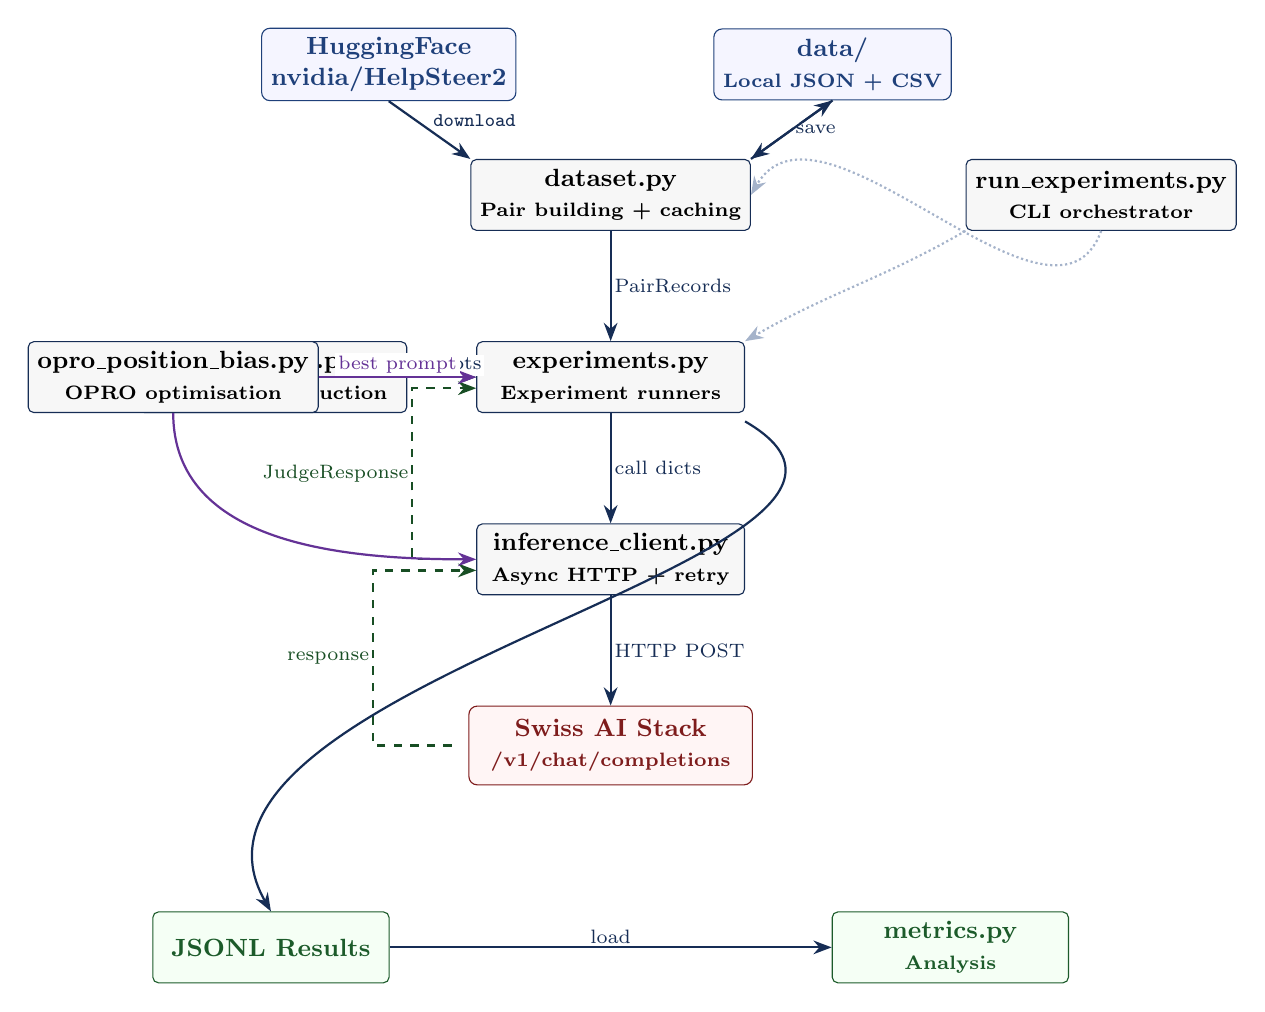
\begin{tikzpicture}[
  >=Stealth,
  node distance=1.0cm and 1.6cm,
  datasrc/.style={
    draw=ethblue, fill=blue!4, rounded corners=3pt,
    minimum width=3.0cm, minimum height=0.9cm,
    font=\small\bfseries, align=center, text=ethblue
  },
  module/.style={
    draw=ethblue!70!black, fill=gray!6, rounded corners=2pt,
    minimum width=3.4cm, minimum height=0.9cm,
    font=\small\bfseries, align=center
  },
  api/.style={
    draw=swissred!70!black, fill=red!4, rounded corners=3pt,
    minimum width=3.6cm, minimum height=1.0cm,
    font=\small\bfseries, align=center, text=swissred!70!black
  },
  output/.style={
    draw=softgreen!70!black, fill=green!4, rounded corners=2pt,
    minimum width=3.0cm, minimum height=0.9cm,
    font=\small\bfseries, align=center, text=softgreen!70!black
  },
  arr/.style={->, thick, ethblue!70!black},
  arrlbl/.style={font=\scriptsize, midway, fill=white, inner sep=1pt},
]

\node[datasrc] (hf1) {HuggingFace\\nvidia/HelpSteer2};
\node[datasrc, right=2.5cm of hf1] (local) {data/\\{\scriptsize Local JSON + CSV}};
\node[module, below=1.2cm of $(hf1)!0.5!(local)$] (dataset) {dataset.py\\{\scriptsize Pair building + caching}};
\node[module, below left=1.4cm and 0.8cm of dataset] (templates) {templates.py\\{\scriptsize Prompt construction}};
\node[module, below=1.4cm of dataset] (experiments) {experiments.py\\{\scriptsize Experiment runners}};
\node[module, below=1.4cm of experiments] (client) {inference\_client.py\\{\scriptsize Async HTTP + retry}};
\node[api, below=1.4cm of client] (swissai) {Swiss AI Stack\\{\scriptsize /v1/chat/completions}};
\node[module, left=2.0cm of experiments] (opro) {opro\_position\_bias.py\\{\scriptsize OPRO optimisation}};
\node[output, below left=1.6cm and 1.0cm of swissai] (jsonl) {JSONL Results};
\node[output, below right=1.6cm and 1.0cm of swissai] (metrics) {metrics.py\\{\scriptsize Analysis}};
\node[module, above right=1.4cm and 2.8cm of experiments] (cli) {run\_experiments.py\\{\scriptsize CLI orchestrator}};

\draw[arr] (hf1.south) -- (dataset.north west) node[arrlbl, above right] {\texttt{download}};
\draw[arr] (dataset.north east) -- (local.south) node[arrlbl, right] {save};
\draw[arr] (local.south) -- (dataset.north east);
\draw[arr] (dataset.south) -- (experiments.north) node[arrlbl, right] {PairRecords};
\draw[arr] (templates.east) -- (experiments.west) node[arrlbl, above] {prompts};
\draw[arr] (experiments.south) -- (client.north) node[arrlbl, right] {call dicts};
\draw[arr] (client.south) -- (swissai.north) node[arrlbl, right] {HTTP POST};
\draw[arr, dashed, softgreen!60!black]
  ([xshift=-6pt]swissai.west) -- +(-1.0,0) |- ([yshift=-4pt]client.west)
  node[arrlbl, pos=0.25, left] {response};
\draw[arr, dashed, softgreen!60!black]
  ([xshift=-6pt]client.west) -- +(-0.6,0) |- ([yshift=-4pt]experiments.west)
  node[arrlbl, pos=0.25, left] {JudgeResponse};
\draw[arr] ([yshift=-3pt]experiments.south east) to[out=-30, in=120] (jsonl.north);
\draw[arr] (jsonl.east) -- (metrics.west) node[arrlbl, above] {load};
\draw[arr, densely dotted, ethblue!40] (cli.south west) to[out=210,in=30] (experiments.north east);
\draw[arr, densely dotted, ethblue!40] (cli.south) to[out=250,in=60] (dataset.east);
\draw[arr, softpurple] (opro.east) -- (experiments.west) node[arrlbl, above] {best prompt};
\draw[arr, softpurple] (opro.south) to[out=-90,in=180] (client.west);

\end{tikzpicture}
\caption{High-level data flow of the evaluation pipeline. Solid arrows
indicate the forward path; dashed arrows show the return path. Purple arrows
represent the OPRO prompt optimisation loop.}
\label{fig:dataflow}
\end{figure}


% ─────────────────────────────────────────────────────────────────────────────
\newpage
\section{Module Descriptions}\label{sec:modules}
% ─────────────────────────────────────────────────────────────────────────────

\subsection{\texttt{dataset.py} --- Data Pipeline}

This module handles all interactions with the HelpSteer2 dataset. The
pipeline operates in two phases:

\paragraph{Download phase.}
The \texttt{download\_dataset()} function fetches HelpSteer2 from HuggingFace,
groups responses by prompt, and constructs \emph{all pairwise combinations}
within each group. For each pair, a composite quality score is computed as
\[
  s = \frac{\text{helpfulness} + \text{correctness} + \text{coherence}}{3}.
\]
The higher-scoring response is placed as~A (gold label~=~``A''); pairs with
equal scores receive gold label~``C''. Results are saved locally as both
JSON and CSV in the \texttt{data/} directory.

Two versions are produced per split:
\begin{itemize}[nosep]
  \item \textbf{Standard}: \texttt{prompt\_id}, \texttt{prompt},
        \texttt{response\_a}, \texttt{response\_b}, \texttt{gold\_label}.
  \item \textbf{Full}: additionally includes per-response scores
        (helpfulness, correctness, coherence, complexity, verbosity for
        both A and B), composite scores, score gap, response lengths, and
        a \texttt{difficulty} label (easy if gap~$> 1.0$, medium if~$> 0.33$,
        hard otherwise).
\end{itemize}

\paragraph{Load phase.}
At experiment time, \texttt{load\_dataset\_pairs()} reads from local JSON,
applies a seeded shuffle, and returns up to~$n$ \texttt{PairRecord} objects.
No network access is required at this stage.

The \texttt{PairRecord} dataclass contains five fields: \texttt{prompt\_id},
\texttt{prompt}, \texttt{response\_a}, \texttt{response\_b}, and
\texttt{gold\_label}. The \texttt{flipped()} method returns a copy with
A and~B swapped and the gold label inverted
($\text{A} \leftrightarrow \text{B}$, $\text{C}$ unchanged).


\subsection{\texttt{inference\_client.py} --- Async HTTP Client}

This module wraps the Swiss~AI~Stack's OpenAI-compatible endpoint with
structured request/response handling, concurrency control, and retry logic.

\paragraph{Configuration.}
The \texttt{InferenceConfig} dataclass holds the endpoint URL, API key, model
identifier, generation parameters (\texttt{max\_tokens}=2048,
\texttt{temperature}=0.0), and retry settings. The model is configurable;
\texttt{check\_models.py} queries the \texttt{/v1/models} endpoint to list
currently available models.

\paragraph{Label extraction.}
After receiving a response, the module extracts the judge verdict through a
three-tier cascade:
\begin{enumerate}[nosep]
  \item Explicit verdict lines (e.g.\ ``Verdict: B'', ``Answer: A'').
  \item A bare A, B, or C at the end of the text.
  \item Fallback: the last standalone A/B/C anywhere in the text.
\end{enumerate}
If the model produced a \texttt{<think>...</think>} block, it is stripped
before extraction and stored separately.

\paragraph{Concurrency and retries.}
The \texttt{SwissAIClient} uses an \texttt{asyncio.Semaphore} (default~8) to
bound the number of concurrent HTTP requests. On rate-limit responses (HTTP~429)
or connection errors, it retries with exponential backoff: delays of 2, 4, 8,
16, 32 seconds, capped at 60~seconds, for up to 5~attempts.


\subsection{\texttt{templates.py} --- Prompt Templates}

All system prompts are defined here and registered in a \texttt{TEMPLATES}
dictionary. Table~\ref{tab:templates} lists the available templates.

\begin{table}[htbp]
\centering
\small
\caption{System prompt templates used across experiments.}
\label{tab:templates}
\begin{tabular}{@{}llc@{}}
  \toprule
  \textbf{Template ID} & \textbf{Framing} & \textbf{Experiment} \\
  \midrule
  \texttt{expert\_rater}  & Baseline expert rater   & B1, B2, B3, B4 \\
  \texttt{llm\_judge}     & ``LLM used to judge''   & B2 \\
  \texttt{neutral}        & Imperative, no persona  & B2 \\
  \texttt{academic}       & Formal quality evaluator & B2 \\
  \texttt{minimal}        & One-liner               & B2 \\
  \texttt{reason\_then\_judge} & Explain reasoning, then verdict & B3 \\
  \texttt{structured\_reasoning} & Rate on criteria, then verdict & B3 \\
  \texttt{expert\_rater\_alt1--3} & Minor wording variants & B4 \\
  \texttt{opro} & OPRO-optimised (low position bias) & B1 \\
  \bottomrule
\end{tabular}
\end{table}

Five evaluation criteria are supported: \texttt{helpful}, \texttt{quality},
\texttt{accurate}, \texttt{harmless}, and \texttt{concise}, each mapping to
a natural-language phrase. The \texttt{build\_prompt()} function resolves a
template ID and criterion into a (system prompt, user prompt) pair. The user
prompt follows a fixed format:

\begin{lstlisting}
[User Prompt]
{prompt}

[Response A]
{response_a}

[Response B]
{response_b}

Which response is {criterion}?
\end{lstlisting}


\subsection{\texttt{experiments.py} --- Experiment Runners}

Four asynchronous functions implement the core experiments. Each builds a list
of call dictionaries, dispatches them via \texttt{batch\_judge()}, and saves
results to JSONL. Table~\ref{tab:experiments} summarises the experimental
conditions.

\begin{table}[htbp]
\centering
\small
\caption{Experiment functions and their conditions.}
\label{tab:experiments}
\begin{tabular}{@{}llp{6.5cm}@{}}
  \toprule
  \textbf{Function} & \textbf{ID} & \textbf{Conditions} \\
  \midrule
  \texttt{run\_position\_bias} & B1 & AB (original), BA (flipped) \\
  \texttt{run\_template\_sensitivity} & B2 & 5 templates \\
  \texttt{run\_reasoning\_depth} & B3 & 3 reasoning conditions \\
  \texttt{run\_input\_sensitivity} & B4 & $4 \times 5 = 20$ (templates $\times$ criteria) \\
  \bottomrule
\end{tabular}
\end{table}


\subsection{\texttt{metrics.py} --- Metric Computation}

This module loads JSONL results and computes experiment-specific metrics:
\begin{itemize}[nosep]
  \item \texttt{compute\_position\_bias}: consistency rate, bias direction,
        and positional preference breakdown.
  \item \texttt{compute\_pairwise\_agreement}: overall and per-pair agreement
        across conditions (used for B2 and B4).
  \item \texttt{compute\_thinking\_accuracy}: accuracy versus gold labels,
        agreement with the no-reasoning baseline, and average latency per
        condition (used for B3).
\end{itemize}


\subsection{CLI Orchestrators}

\paragraph{\texttt{run\_experiments.py}} is the main entry point. It loads
the dataset, configures the inference client, runs selected experiments,
computes metrics, and prints summaries. Key flags include
\texttt{--experiments}, \texttt{--n-pairs}, \texttt{--template} (including
\texttt{opro}), \texttt{--model}, and \texttt{--concurrency}.

\paragraph{\texttt{run\_opro.py}} runs the OPRO optimisation loop
(Section~\ref{sec:opro}). It loads training and validation pairs, invokes
the optimiser, and prints the best prompt with its scores.

\paragraph{\texttt{check\_models.py}} queries the \texttt{/v1/models} endpoint
and lists all currently available models on the Swiss~AI~Stack---useful since
model availability changes frequently.


% ─────────────────────────────────────────────────────────────────────────────
\newpage
\section{Experiments}\label{sec:experiments}
% ─────────────────────────────────────────────────────────────────────────────

\subsection{B1: Position Bias}\label{sec:b1}

\paragraph{Research question.}
Does the LLM judge prefer whichever response appears in a particular position,
regardless of content quality?

\paragraph{Method.}
For each pair, the judge is queried twice: once with the original ordering
(condition~AB) and once with responses swapped (condition~BA). A consistent
judge should prefer the same underlying response in both orderings---if the
AB~verdict is ``A'', the BA~verdict should be ``B''.

\paragraph{Metrics.}
\begin{itemize}[nosep]
  \item \textit{Position consistency}: fraction of pairs where the flipped
        verdict matches the expected inversion.
  \item \textit{Bias toward first/second position}: fraction where the model
        always selects the response in position~A (or~B), regardless of content.
  \item \textit{Tie inconsistency}: cases where one ordering produces a tie
        and the other does not.
\end{itemize}


\subsection{B2: Template Sensitivity}\label{sec:b2}

\paragraph{Research question.}
How sensitive is the judge's verdict to the framing of the system prompt,
given identical data and response ordering?

\paragraph{Method.}
Each pair is judged with five system prompt templates (Table~\ref{tab:templates}),
keeping data, order, and criterion constant. Only the judge persona changes.

\paragraph{Metrics.}
Overall pairwise agreement across templates, label distribution per template,
and identification of the most volatile pairs (lowest cross-template agreement).


\subsection{B3: Reasoning Depth}\label{sec:b3}

\paragraph{Research question.}
Does explicitly prompting the model to reason before giving its verdict improve
accuracy against human gold labels?

\paragraph{Method.}
Three conditions are compared, differing only in the system prompt:
\begin{enumerate}[nosep]
  \item \textit{No reasoning}: output only A, B, or C.
  \item \textit{Reason then judge}: explain strengths and weaknesses, then
        give a verdict.
  \item \textit{Structured reasoning}: rate each response on helpfulness,
        accuracy, and coherence, then give a verdict.
\end{enumerate}
All reasoning is prompt-elicited---the prompt itself requests the reasoning.
No native API thinking-budget feature is used.

\paragraph{Metrics.}
Accuracy versus gold labels per condition, delta accuracy over the
no-reasoning baseline, and average latency (reasoning conditions produce
longer outputs).


\subsection{B4: Input Sensitivity}\label{sec:b4}

\paragraph{Research question.}
How sensitive is the judge to minor paraphrasing of the system prompt and
changes in the evaluation criterion?

\paragraph{Method.}
Four semantically equivalent variants of the \texttt{expert\_rater} template
are crossed with five evaluation criteria, yielding $4 \times 5 = 20$
conditions per pair.

\paragraph{Metrics.}
Pairwise agreement across conditions and criterion drift (how much the
label changes when only the criterion changes, with the template held fixed).


% ─────────────────────────────────────────────────────────────────────────────
\subsection{OPRO: Prompt Optimisation for Position Bias}\label{sec:opro}
% ─────────────────────────────────────────────────────────────────────────────

\paragraph{Goal.}
Automatically discover a system prompt that minimises position bias, using
the LLM itself to iteratively generate and refine candidates.

\paragraph{Method.}
The optimisation follows the OPRO framework (Optimization by PROmpting):
\begin{enumerate}[nosep]
  \item Evaluate two seed prompts (\texttt{expert\_rater} and
        \texttt{llm\_judge}) on a fixed subset of training pairs, measuring
        position consistency.
  \item For $N$~iterations: present the LLM with the full history of
        (prompt~$\to$~score) pairs and ask it to generate a new system prompt.
        Evaluate the candidate on the same training subset.
  \item Select the prompt with the highest training score.
  \item Validate on a held-out set to assess generalisation.
\end{enumerate}

A fixed subset of training pairs (default~80) is used for all evaluations,
ensuring that scores are comparable across iterations. The best prompt is
saved to \texttt{results/opro/opro\_results.json} and registered as the
\texttt{opro} template.

\paragraph{Transferability.}
OPRO-generated prompts are model-specific. A prompt optimised for one model
(e.g.\ Qwen) may not generalise to another (e.g.\ Llama), as different
architectures respond differently to debiasing instructions. When switching
models, the optimisation should be re-run.

\begin{lstlisting}[title={\small OPRO usage}]
# Default: 10 iterations, 80 eval pairs, 150 validation pairs
python run_opro.py

# Use the optimised prompt in experiments
python run_experiments.py --template opro --experiments position_bias
\end{lstlisting}


% ─────────────────────────────────────────────────────────────────────────────
\newpage
\section{Concurrency and Retry Logic}\label{sec:concurrency}
% ─────────────────────────────────────────────────────────────────────────────

The pipeline uses Python's \texttt{asyncio} event loop with \texttt{aiohttp}
for non-blocking HTTP. All experiment calls are dispatched simultaneously
via \texttt{asyncio.gather()}, bounded by an \texttt{asyncio.Semaphore}.

\paragraph{Concurrency control.}
The semaphore (default~8) ensures that at most 8~HTTP requests are in flight
at any time, preventing server overload while maintaining high throughput.

\paragraph{Exponential backoff.}
On HTTP~429 (rate limit) or connection errors, the client waits
$\min(\text{base\_delay} \times 2^{\text{attempt}},\; 60)$~seconds before
retrying. With a base delay of~2\,s, the sequence is 2, 4, 8, 16, 32\,s
(capped at~60\,s). After 5~failed attempts, a \texttt{RuntimeError} is raised.

Figure~\ref{fig:retry} illustrates the retry flow.

\begin{figure}[htbp]
\centering
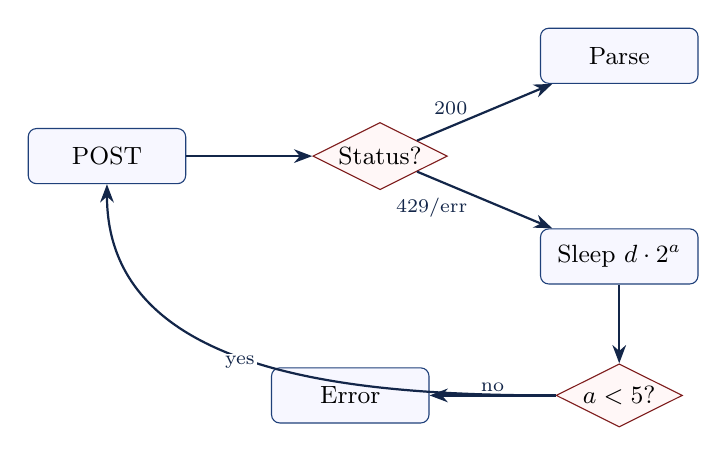
\begin{tikzpicture}[
  >=Stealth,
  state/.style={draw=ethblue, fill=blue!3, rounded corners=3pt,
                minimum width=2.0cm, minimum height=0.7cm,
                font=\small, align=center},
  decision/.style={draw=swissred!70!black, fill=red!3,
                   diamond, aspect=2, inner sep=1pt,
                   font=\small, align=center},
  arr/.style={->, thick, ethblue!60!black},
  lbl/.style={font=\scriptsize, fill=white, inner sep=1pt},
]

\node[state] (req) {POST};
\node[decision, right=1.6cm of req] (check) {Status?};
\node[state, above right=0.7cm and 1.6cm of check] (ok) {Parse};
\node[state, below right=0.7cm and 1.6cm of check] (wait) {Sleep $d \cdot 2^a$};
\node[decision, below=1.0cm of wait] (retry) {$a < 5$?};
\node[state, left=1.6cm of retry] (fail) {Error};

\draw[arr] (req) -- (check);
\draw[arr] (check) -- (ok) node[lbl, pos=0.4, above left] {200};
\draw[arr] (check) -- (wait) node[lbl, pos=0.4, below left] {429/err};
\draw[arr] (wait) -- (retry);
\draw[arr] (retry.west) -- (fail) node[lbl, midway, above] {no};
\draw[arr] (retry.west) to[out=180, in=270] node[lbl, pos=0.5, left] {yes} (req.south);

\end{tikzpicture}
\caption{Exponential backoff retry logic. On rate-limit or error responses,
the client retries up to 5~times with increasing delays.}
\label{fig:retry}
\end{figure}


% ─────────────────────────────────────────────────────────────────────────────
\newpage
\section{Output Format}\label{sec:output}
% ─────────────────────────────────────────────────────────────────────────────

Each experiment writes a JSONL file to the \texttt{results/} directory, with
one JSON object per judge call. Table~\ref{tab:fields} describes the schema.

\begin{table}[htbp]
\centering
\small
\caption{Fields in each JSONL result record.}
\label{tab:fields}
\begin{tabular}{@{}llp{7cm}@{}}
  \toprule
  \textbf{Field} & \textbf{Type} & \textbf{Description} \\
  \midrule
  \texttt{prompt\_id} & str & Unique identifier for the dataset pair \\
  \texttt{experiment\_id} & str & Experiment name \\
  \texttt{condition} & str & Experimental condition (e.g.\ AB, BA, template name) \\
  \texttt{raw\_text} & str & Full model output, unmodified \\
  \texttt{label} & str\,|\,null & Extracted verdict: A, B, C, or null \\
  \texttt{thinking} & str\,|\,null & Extracted reasoning block, if present \\
  \texttt{latency\_s} & float & Request latency in seconds \\
  \texttt{total\_tokens} & int & Total tokens (prompt + completion) \\
  \texttt{parse\_ok} & bool & Whether label extraction succeeded \\
  \texttt{error} & str\,|\,null & Error message, if the request failed \\
  \bottomrule
\end{tabular}
\end{table}

The results directory is organised as follows:

\begin{lstlisting}
results/
  position_bias/
    expert_rater_helpful.jsonl
    opro_helpful.jsonl
  template_sensitivity/
    criterion_helpful.jsonl
  reasoning_depth/
    criterion_helpful.jsonl
  input_sensitivity/
    all.jsonl
  opro/
    opro_results.json
\end{lstlisting}


% ─────────────────────────────────────────────────────────────────────────────
\section{Infrastructure}\label{sec:infra}
% ─────────────────────────────────────────────────────────────────────────────

This pipeline performs no local GPU inference. All model calls are HTTP
requests to the Swiss~AI~Stack. Table~\ref{tab:infra} summarises the
infrastructure.

\begin{table}[htbp]
\centering
\small
\caption{Infrastructure summary.}
\label{tab:infra}
\begin{tabular}{@{}ll@{}}
  \toprule
  \textbf{Component} & \textbf{Detail} \\
  \midrule
  Inference backend & Swiss AI Stack (CSCS) \\
  Endpoint & \url{https://api.swissai.cscs.ch/v1} \\
  API compatibility & OpenAI \texttt{/v1/chat/completions} \\
  Model & Configurable (use \texttt{check\_models.py}) \\
  Authentication & Bearer token via \texttt{SWISSAI\_API\_KEY} \\
  Client library & \texttt{aiohttp} (async) \\
  Concurrency & Semaphore-bounded (default 8) \\
  Retry strategy & Exponential backoff, max 5 retries \\
  Local requirements & Python 3.10+, aiohttp, datasets, numpy \\
  Local GPU / cluster & None \\
  \bottomrule
\end{tabular}
\end{table}


% ─────────────────────────────────────────────────────────────────────────────
\newpage
\section{Dataset Analysis}\label{sec:analysis}
% ─────────────────────────────────────────────────────────────────────────────

The following figures are generated by \texttt{dataset\_analysis.ipynb} and
provide an overview of the HelpSteer2 dataset used in all experiments.

\subsection{Rating Distributions and Correlations}

\begin{figure}[htbp]
\centering
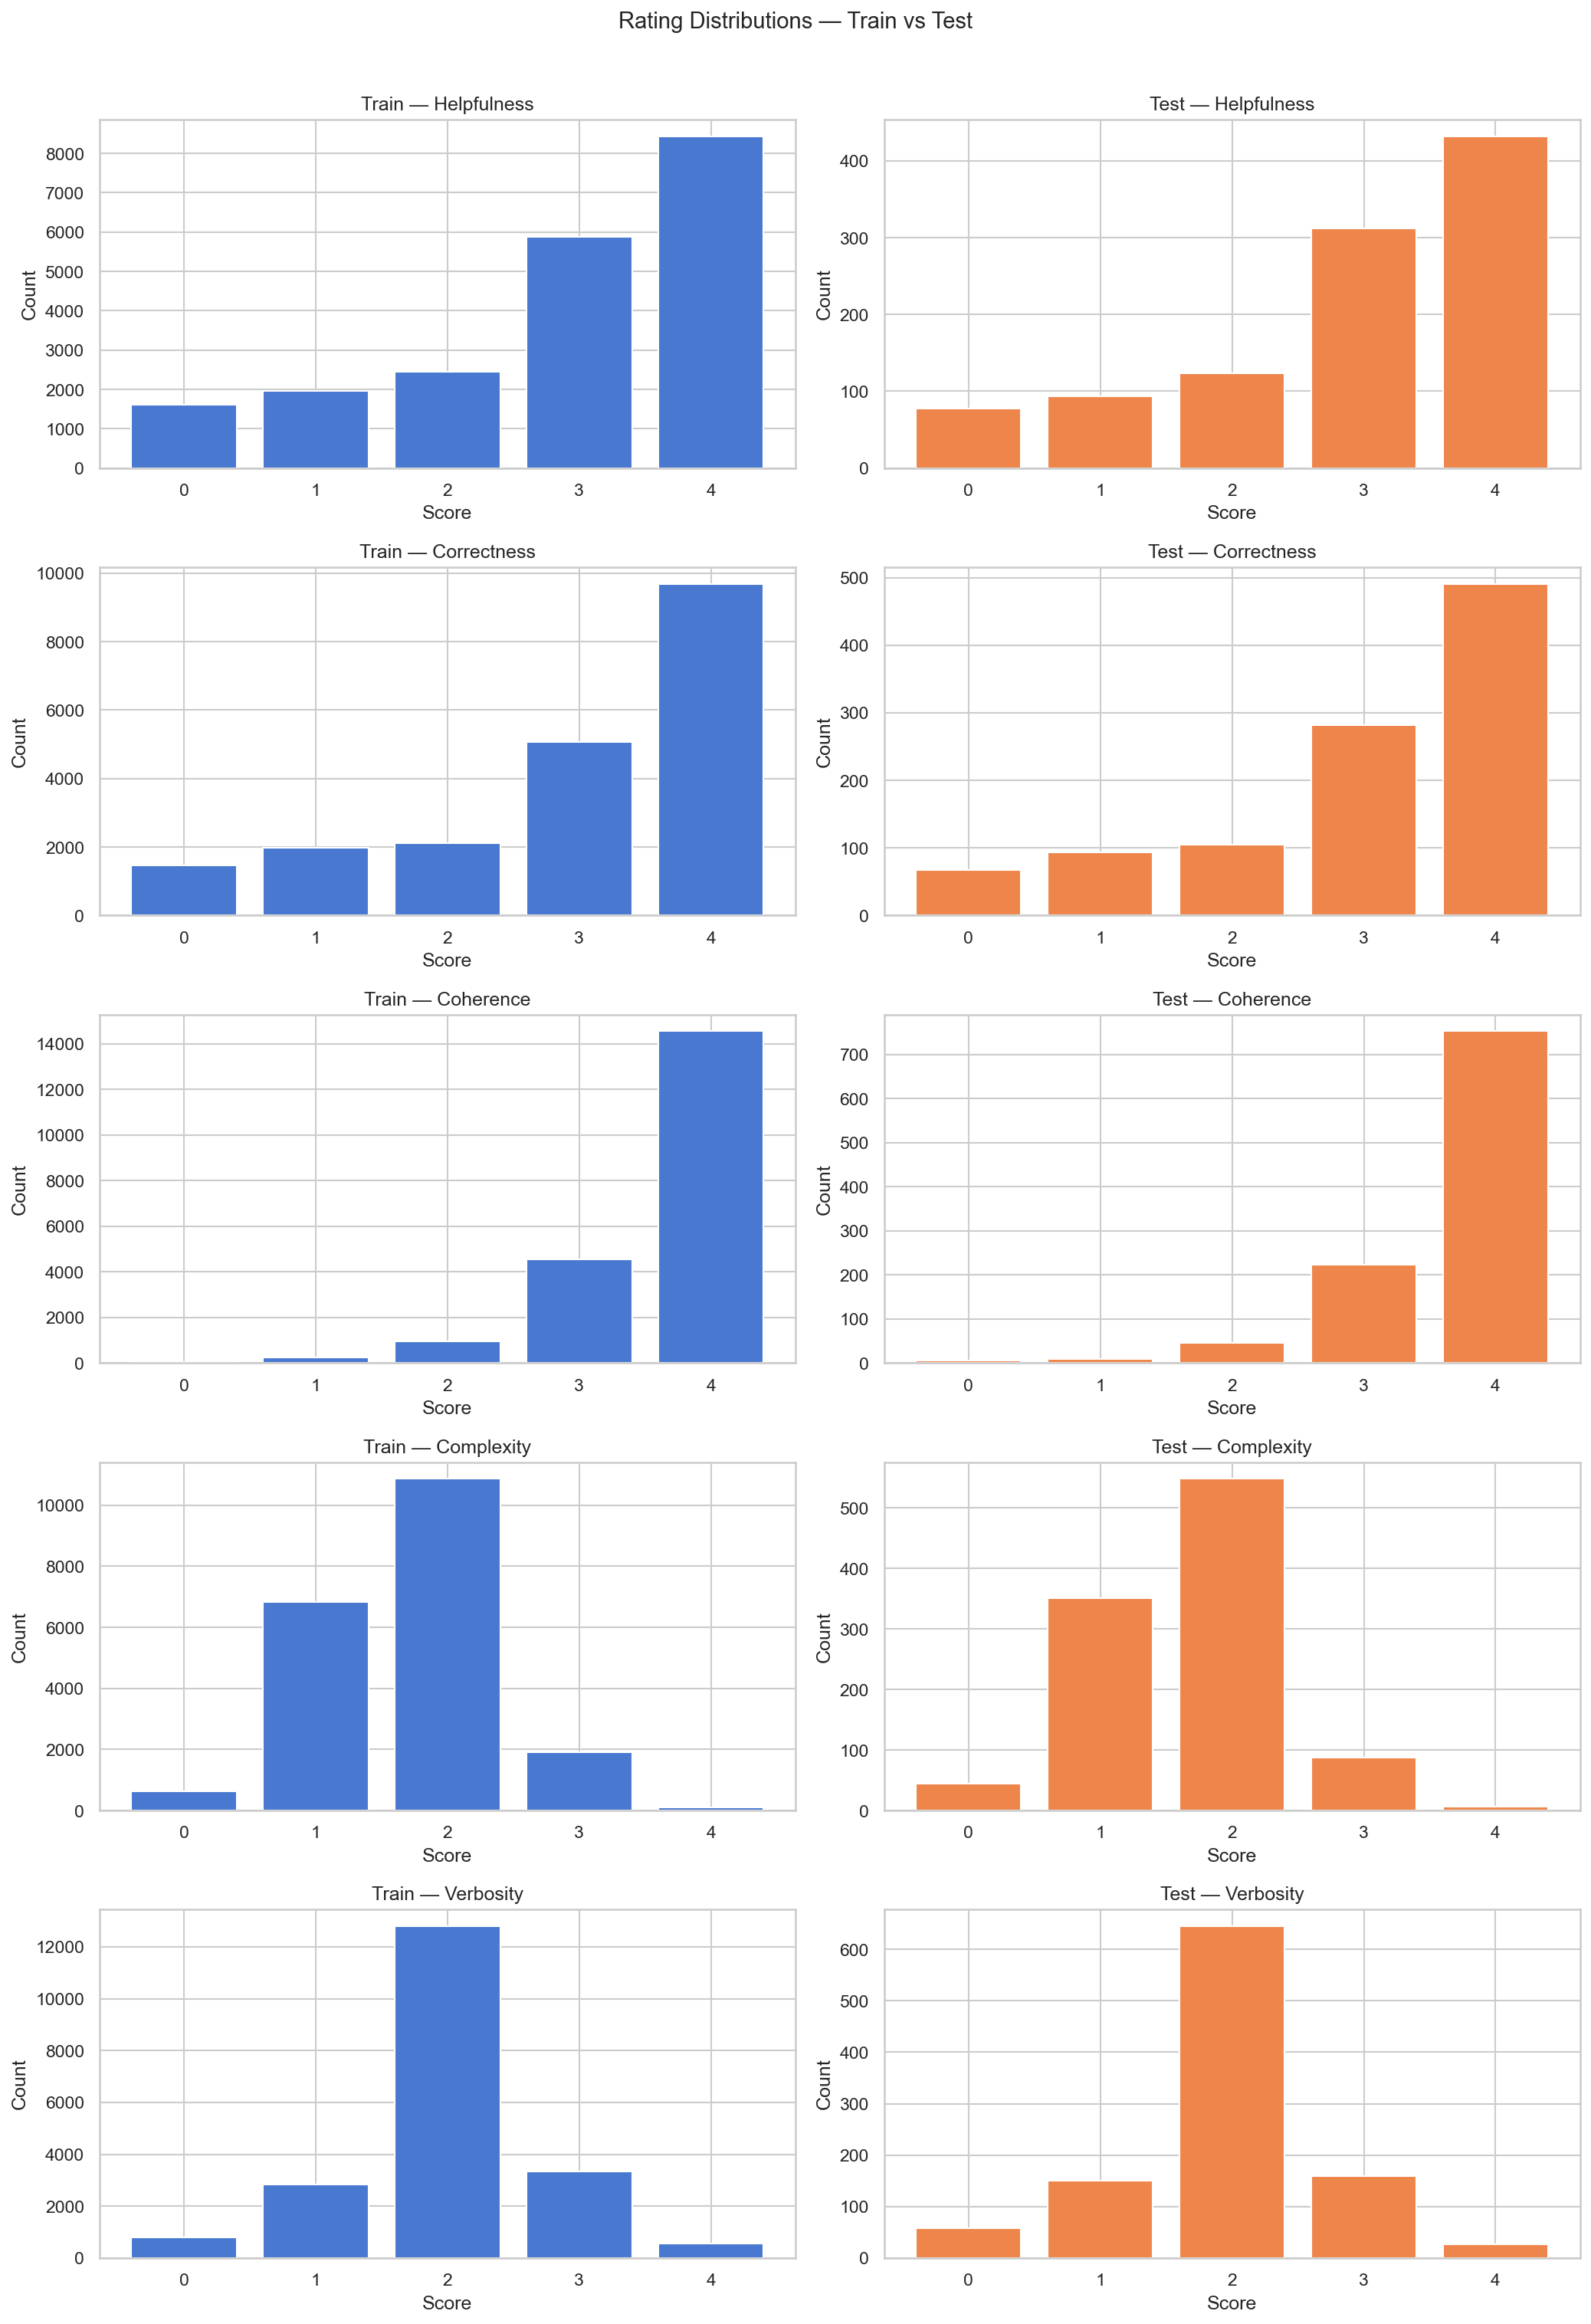
\includegraphics[width=0.5\textwidth]{figures/rating_distributions.png}
\caption{Distribution of helpfulness, correctness, coherence, complexity,
and verbosity ratings across all responses.}
\label{fig:ratings}
\end{figure}

\begin{figure}[htbp]
\centering
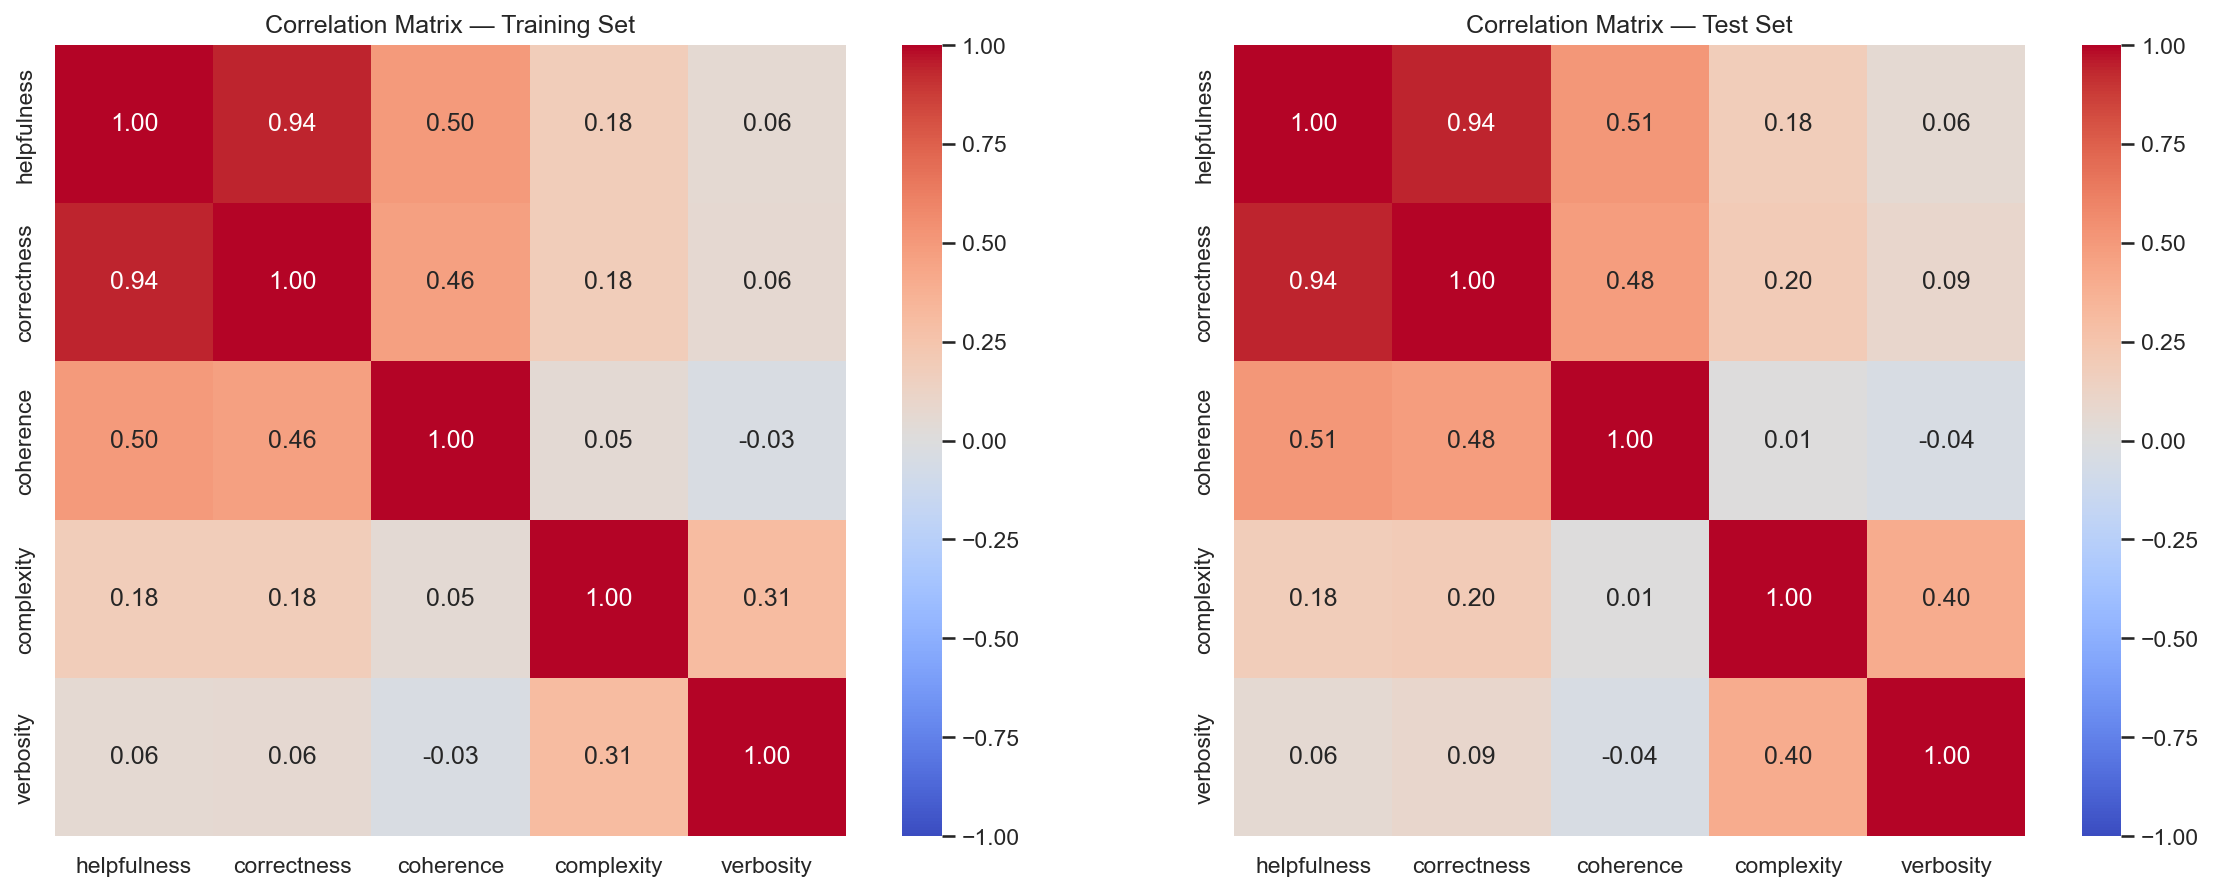
\includegraphics[width=0.6\textwidth]{figures/metric_correlation_heatmap.png}
\caption{Pairwise Pearson correlation between rating dimensions. Helpfulness
and correctness are strongly correlated, suggesting these criteria capture
overlapping aspects of response quality.}
\label{fig:correlation}
\end{figure}
\newpage
\subsection{Response Length}

\begin{figure}[htbp]
\centering
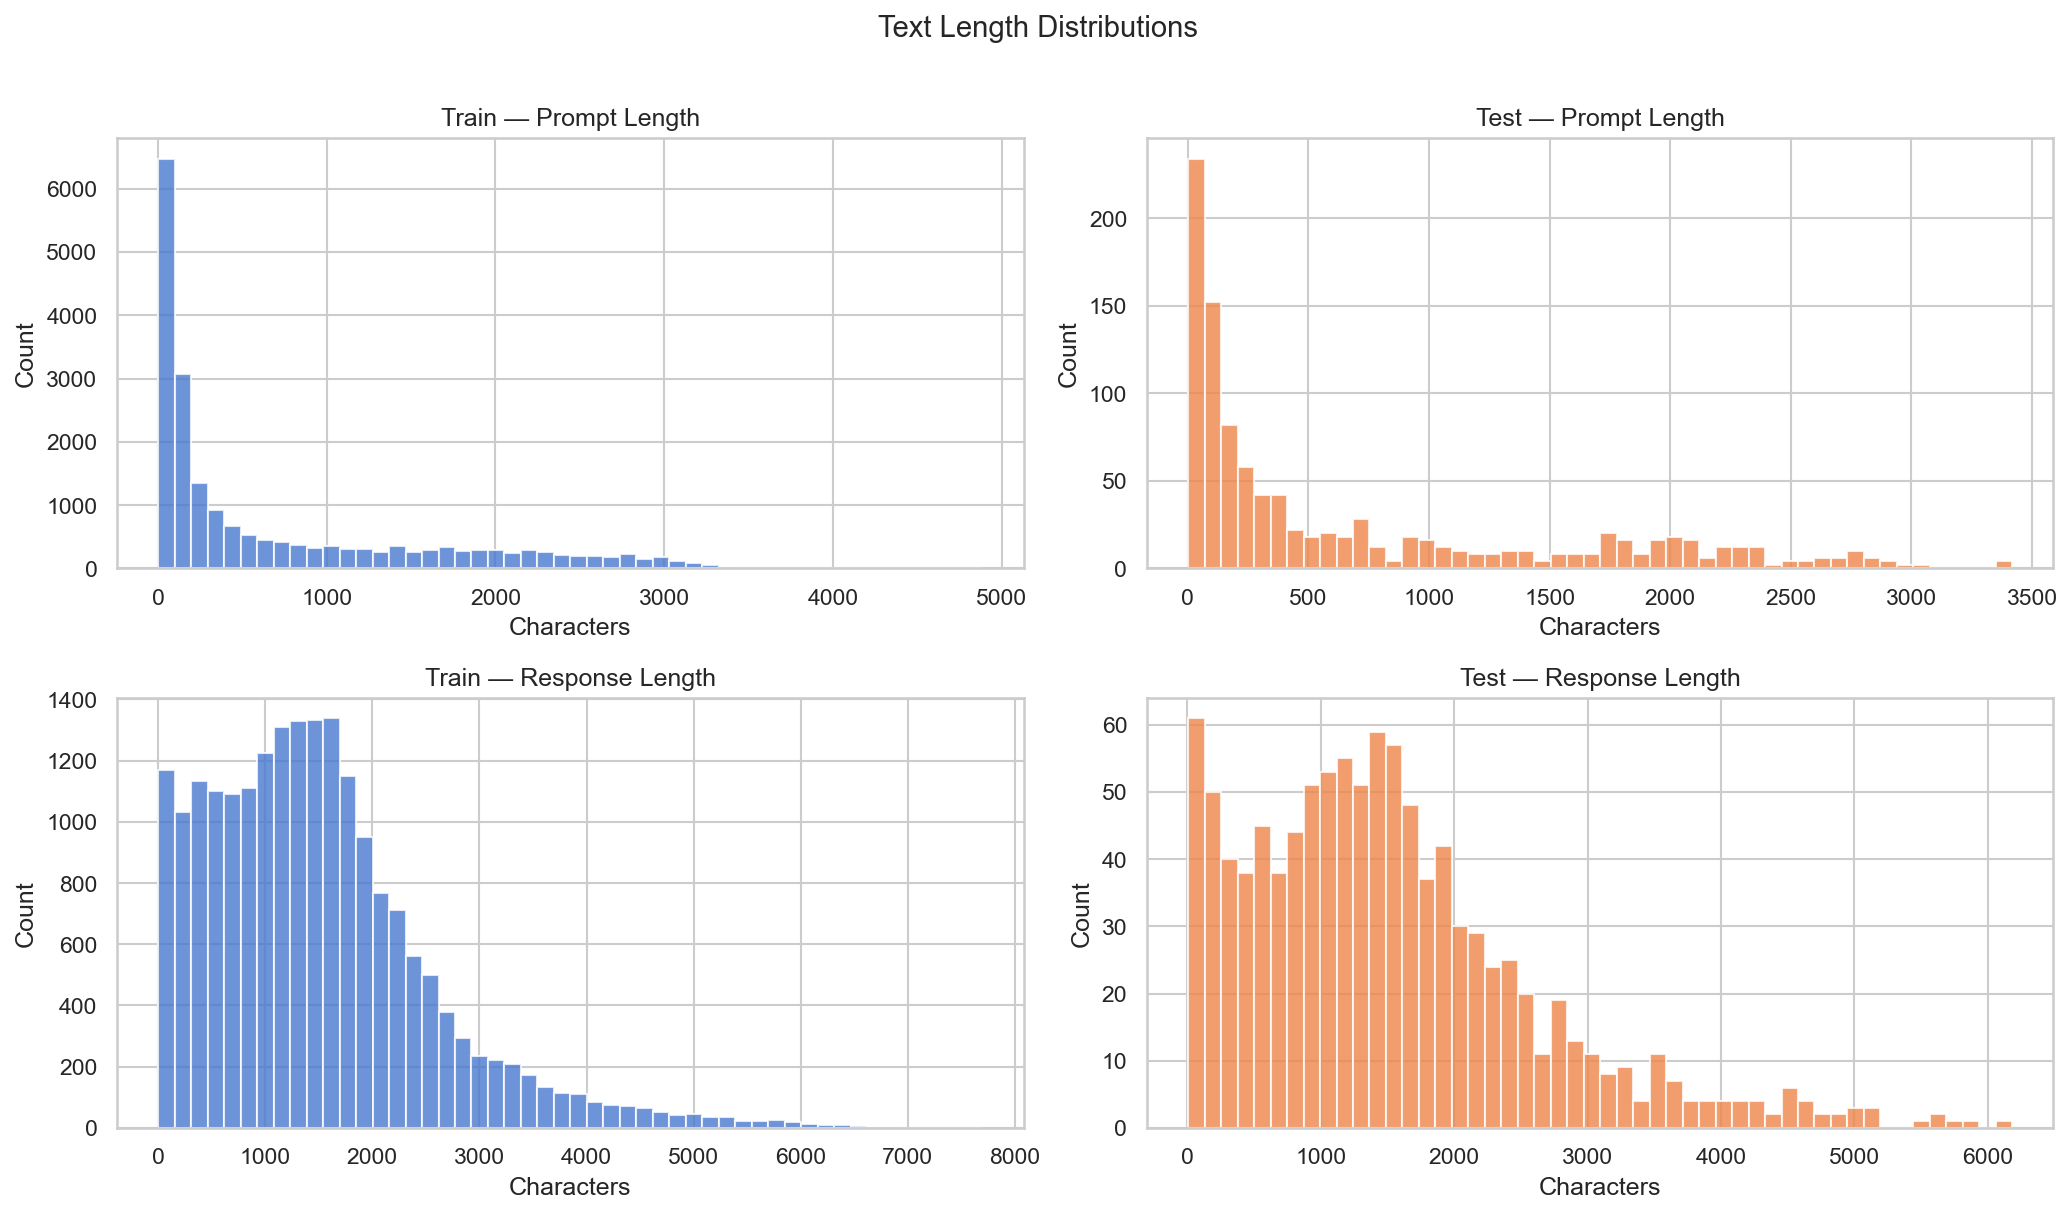
\includegraphics[width=0.6\textwidth]{figures/text_length_distributions.png}
\caption{Distribution of prompt and response lengths (in characters).}
\label{fig:lengths}
\end{figure}

\begin{figure}[htbp]
\centering
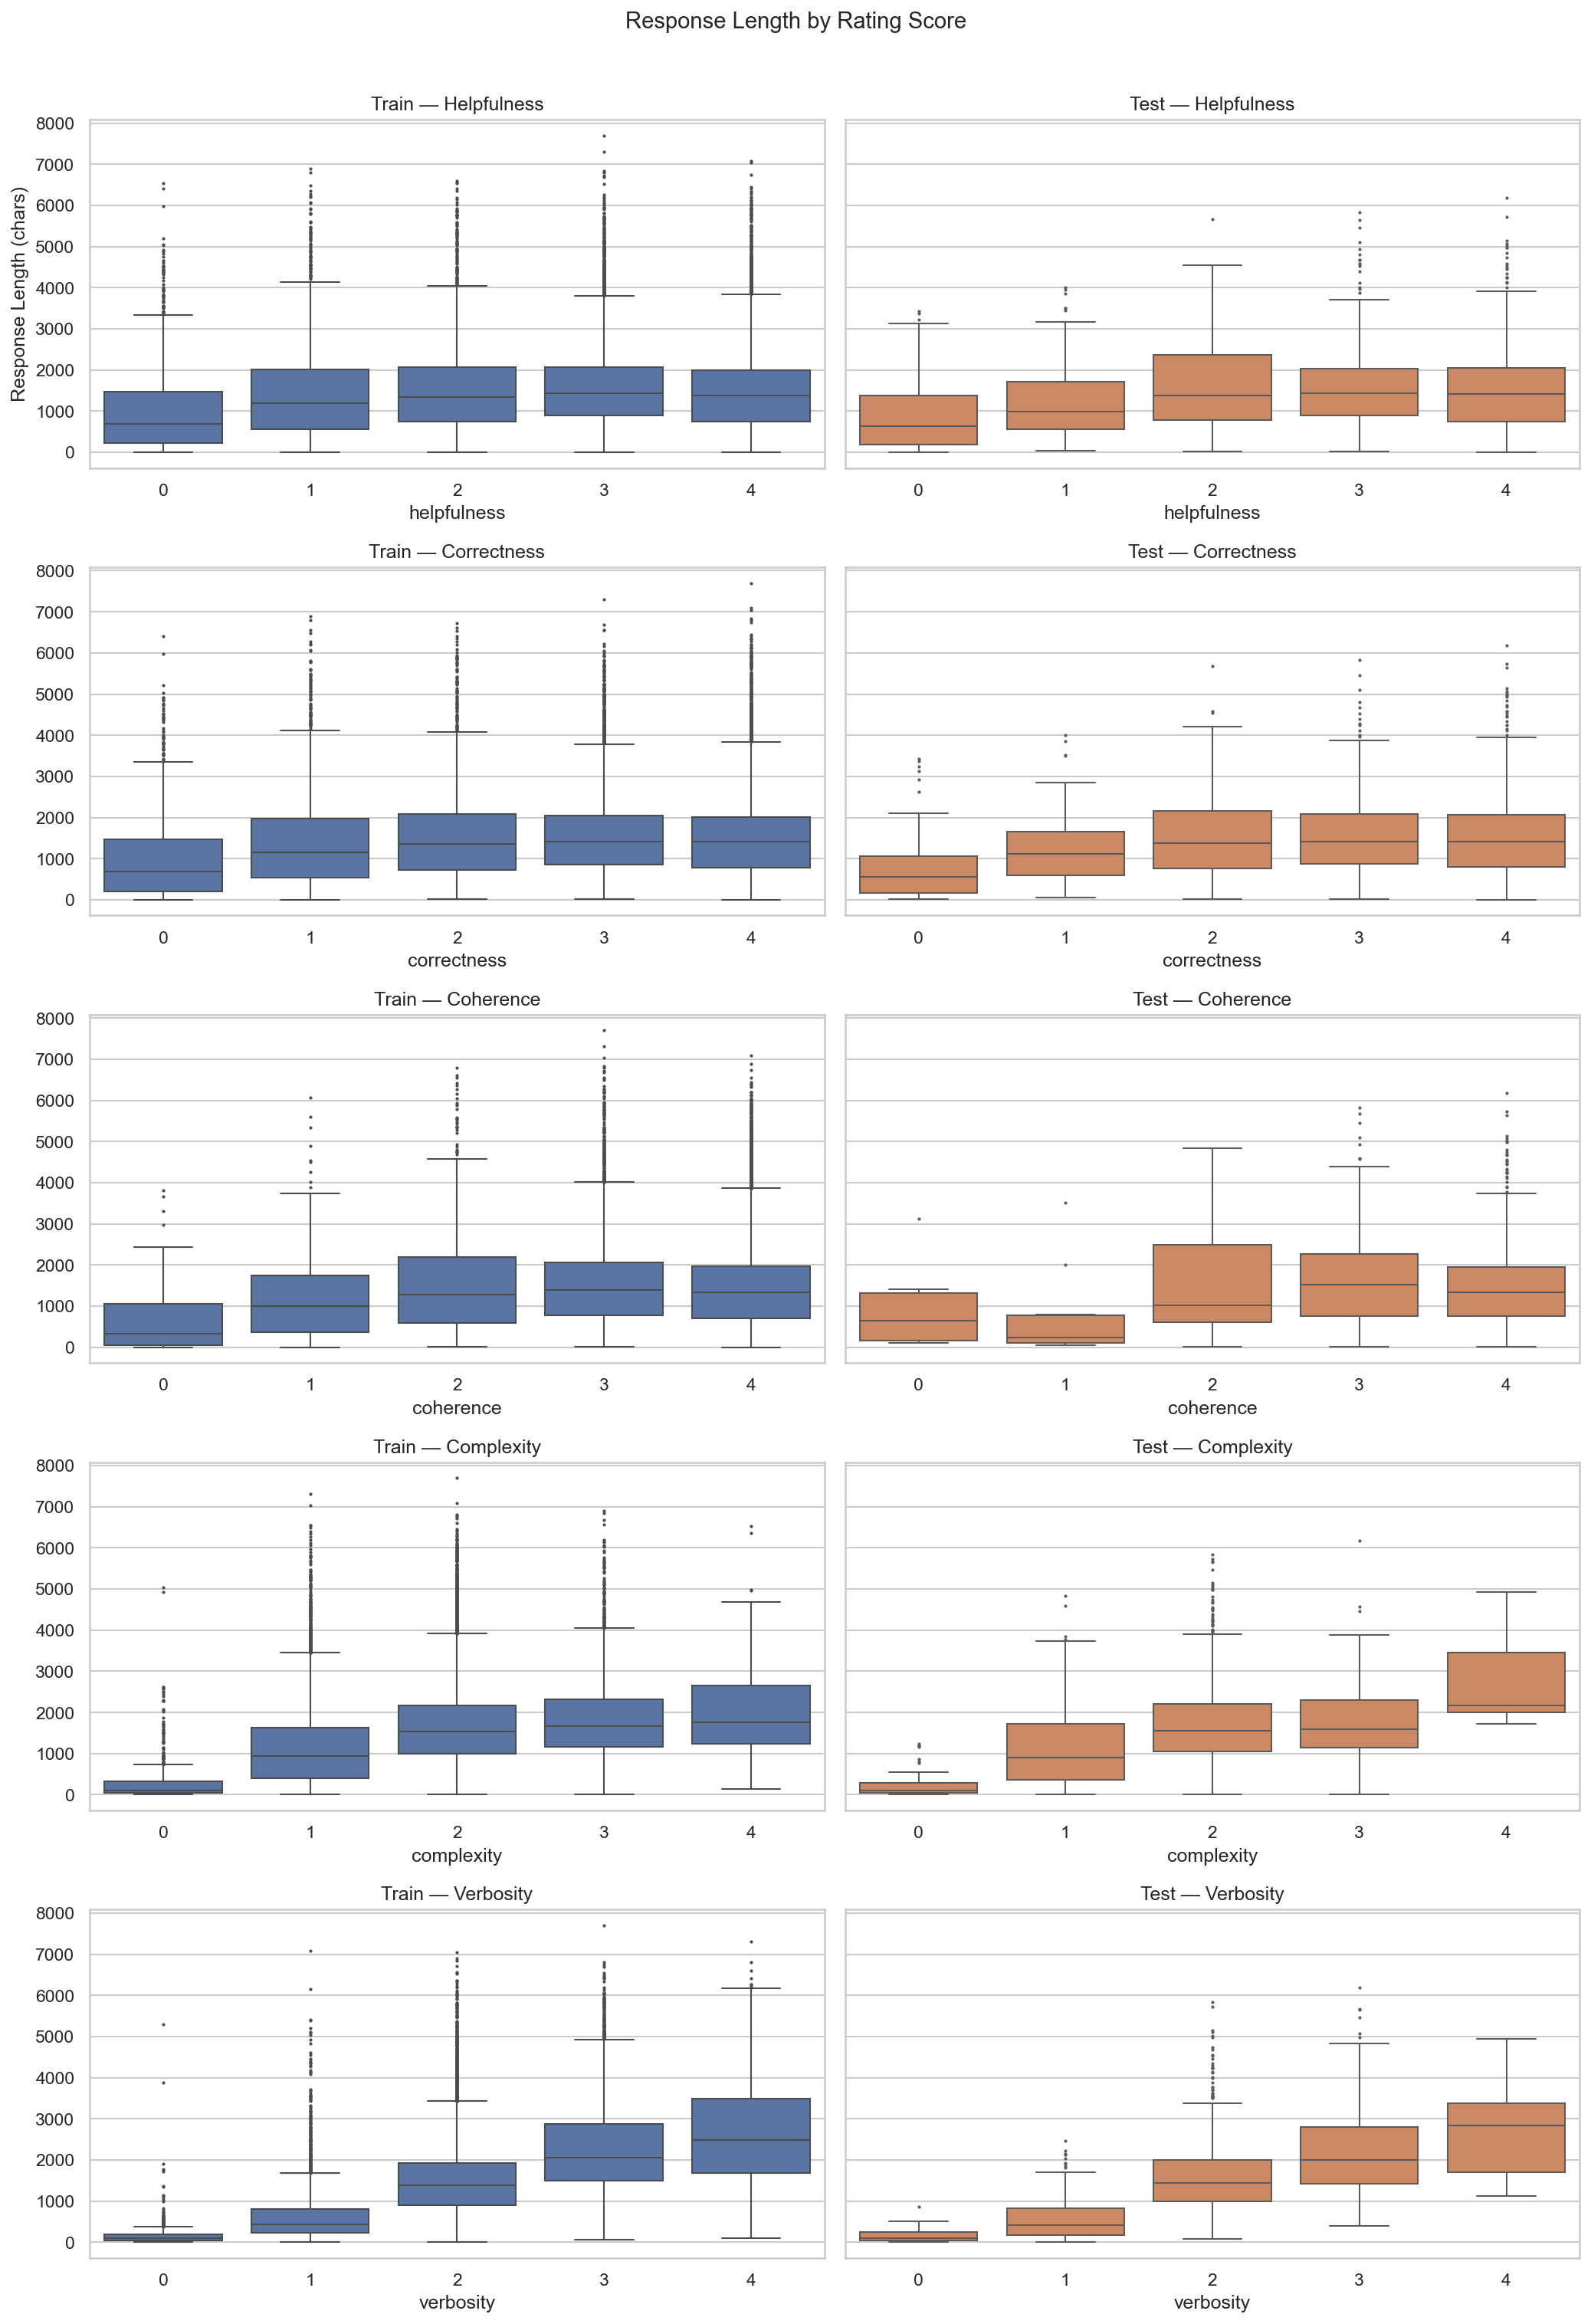
\includegraphics[width=0.45\textwidth]{figures/response_length_by_rating.png}
\caption{Response length by helpfulness rating. Longer responses tend to
receive higher scores.}
\label{fig:length_rating}
\end{figure}

\newpage
\subsection{Metric Gaps Between Paired Responses}

\begin{figure}[htbp]
\centering
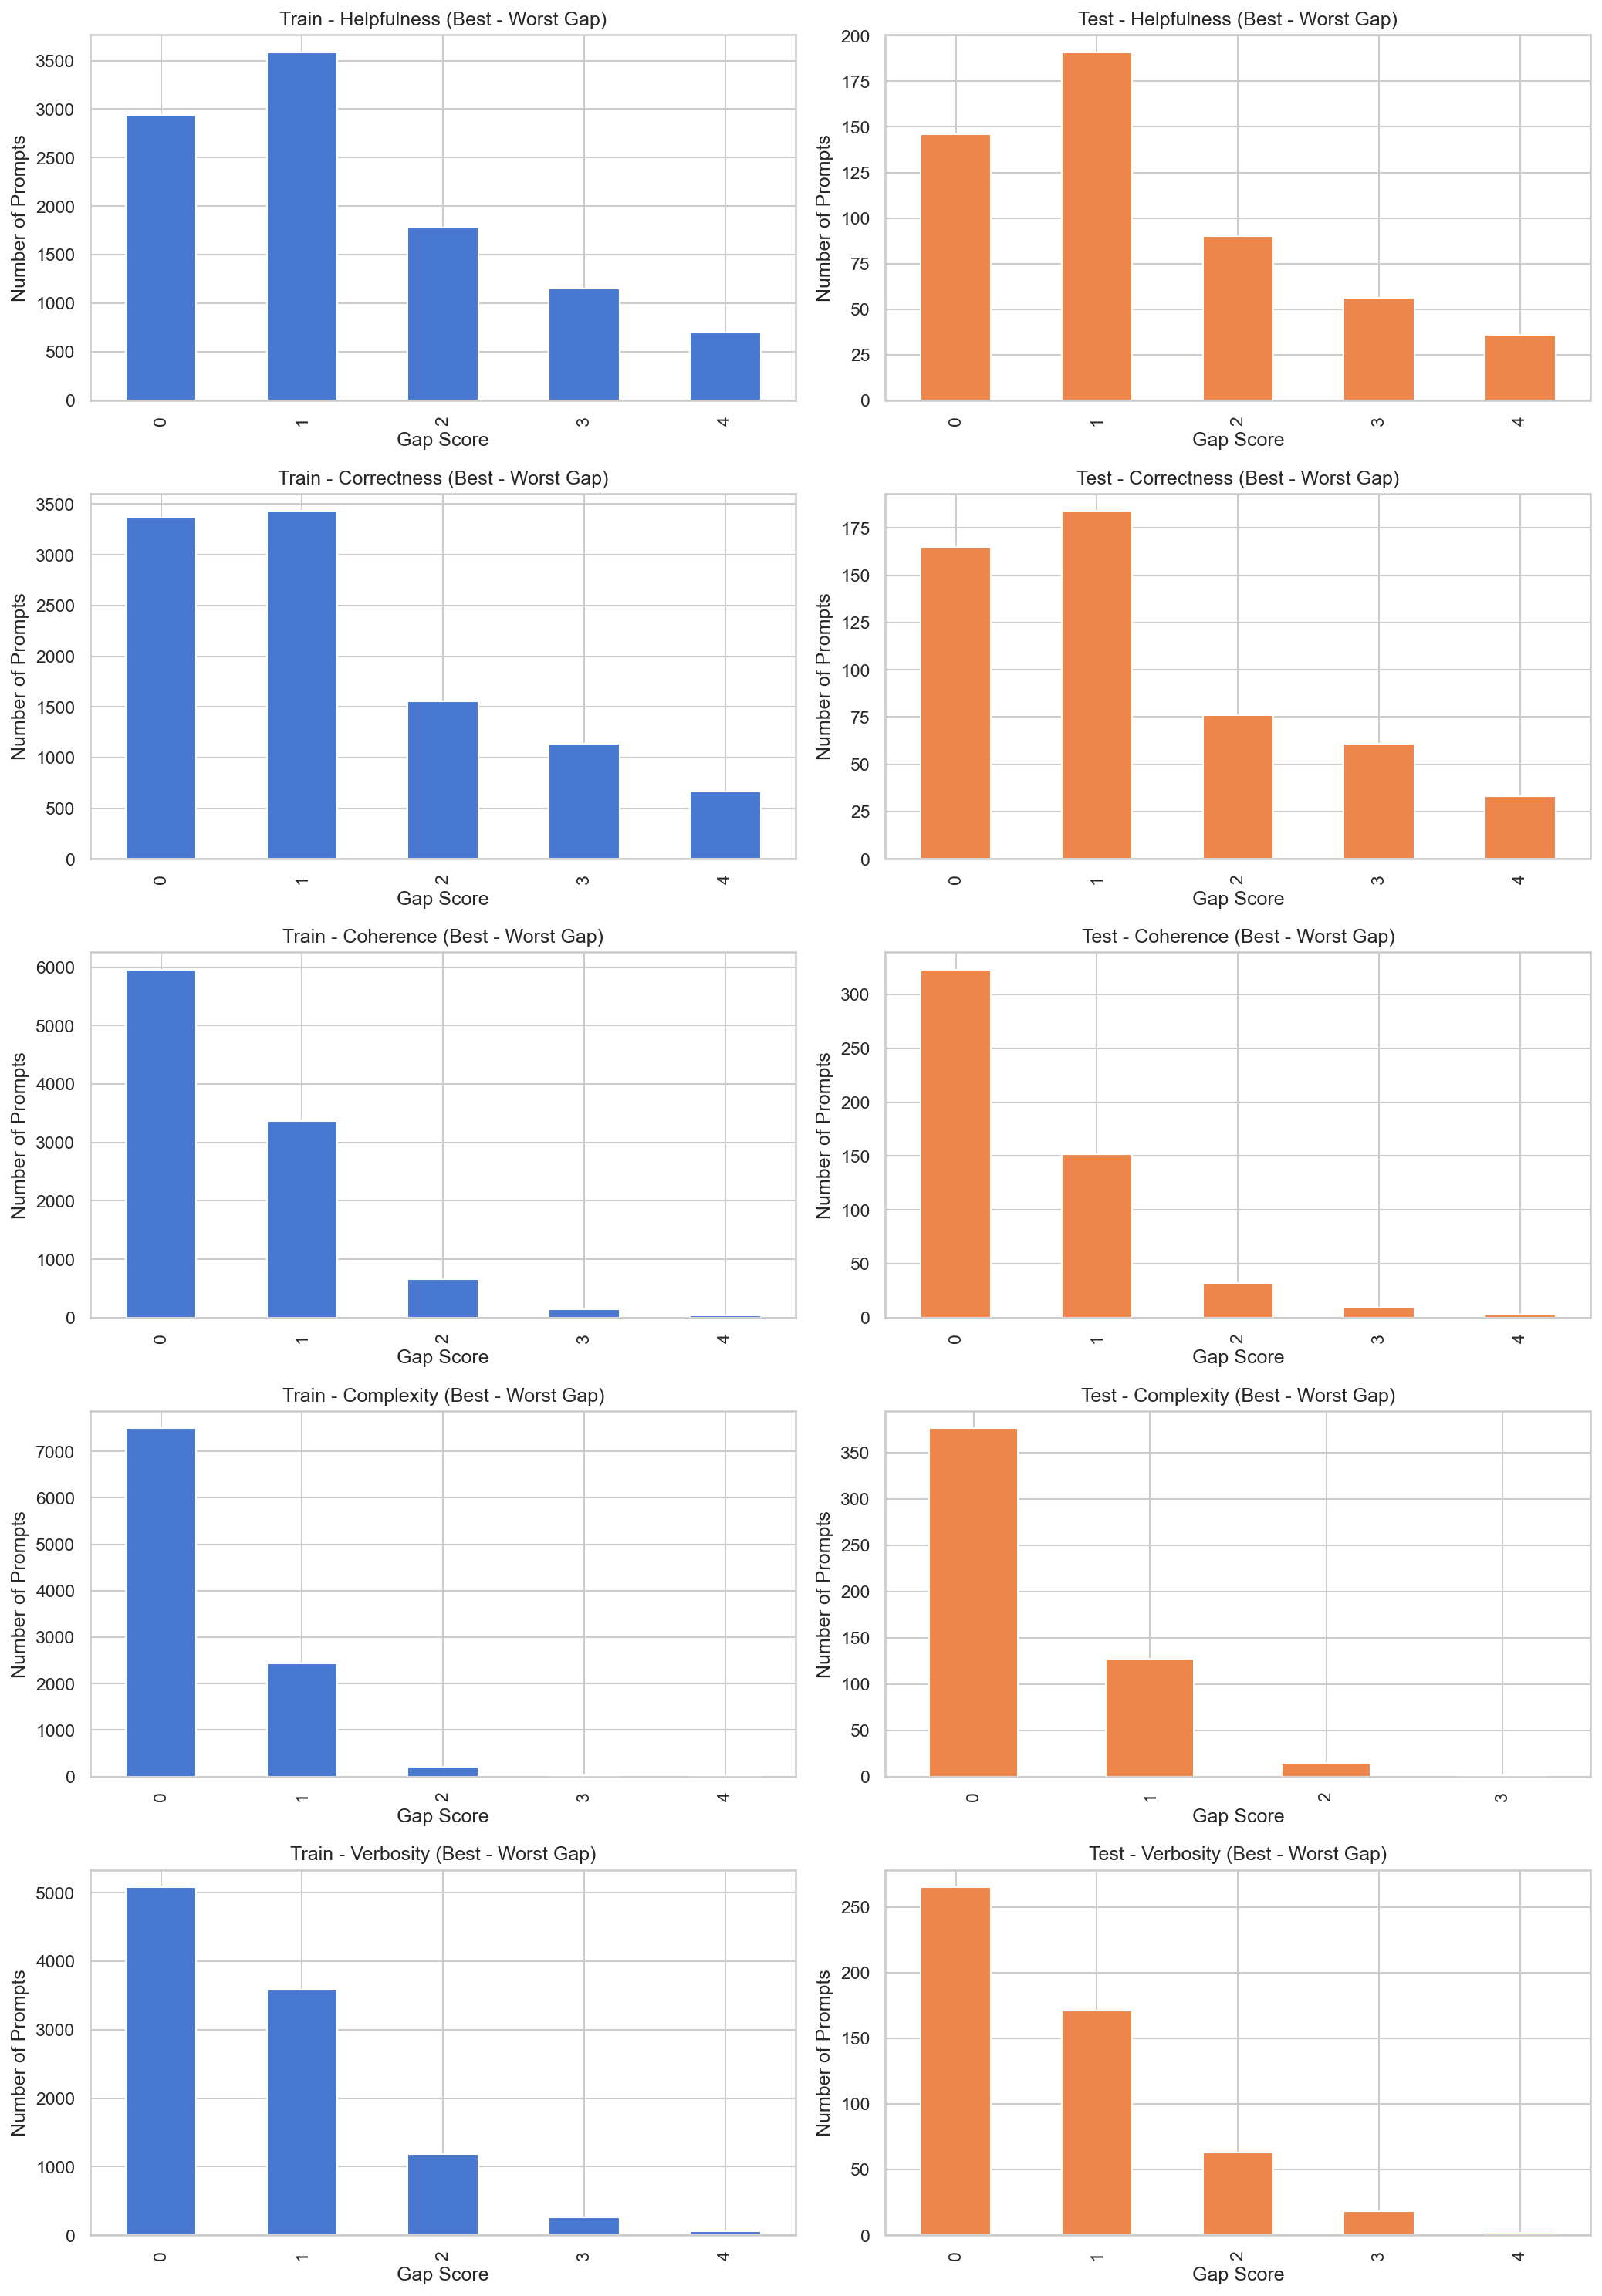
\includegraphics[width=0.45\textwidth]{figures/metric_gap_distributions.png}
\caption{Distribution of per-metric gaps (score of A minus score of B) across
all pairs. Larger gaps correspond to easier judgments.}
\label{fig:gaps}
\end{figure}

\begin{figure}[htbp]
\centering
\begin{minipage}{0.5\textwidth}
  \centering
  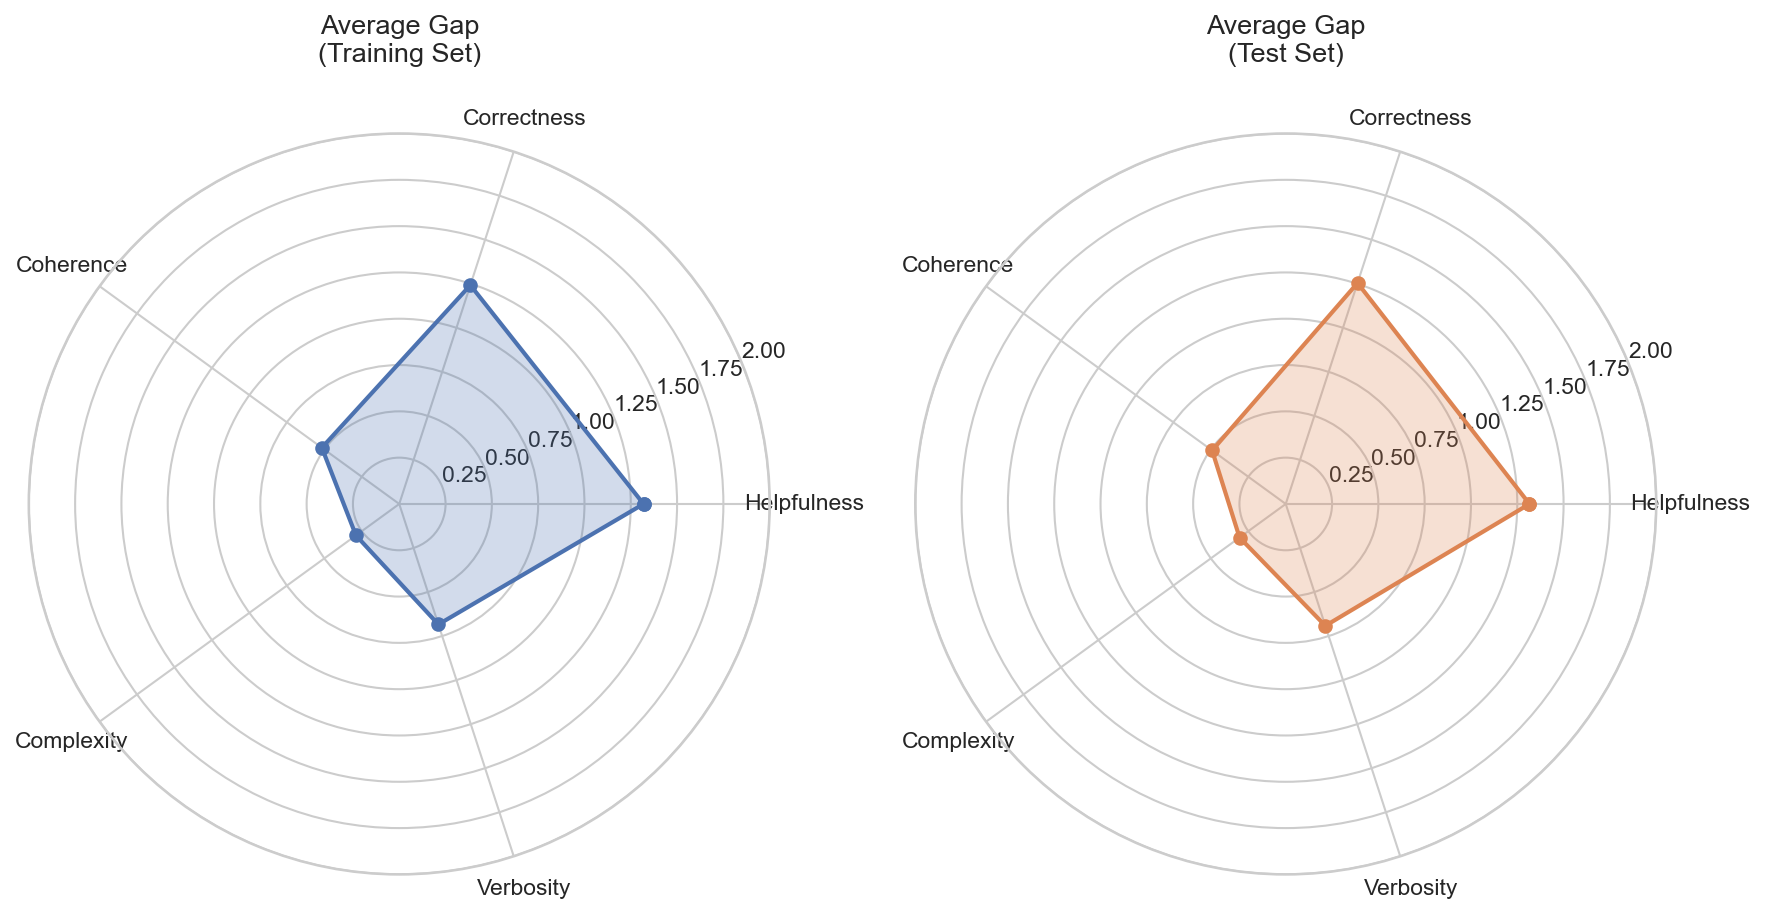
\includegraphics[width=\textwidth]{figures/average_gap_radar.png}
  \captionof{figure}{Average metric gaps.}
  \label{fig:gap_radar}
\end{minipage}\hfill
\begin{minipage}{0.48\textwidth}
  \centering
  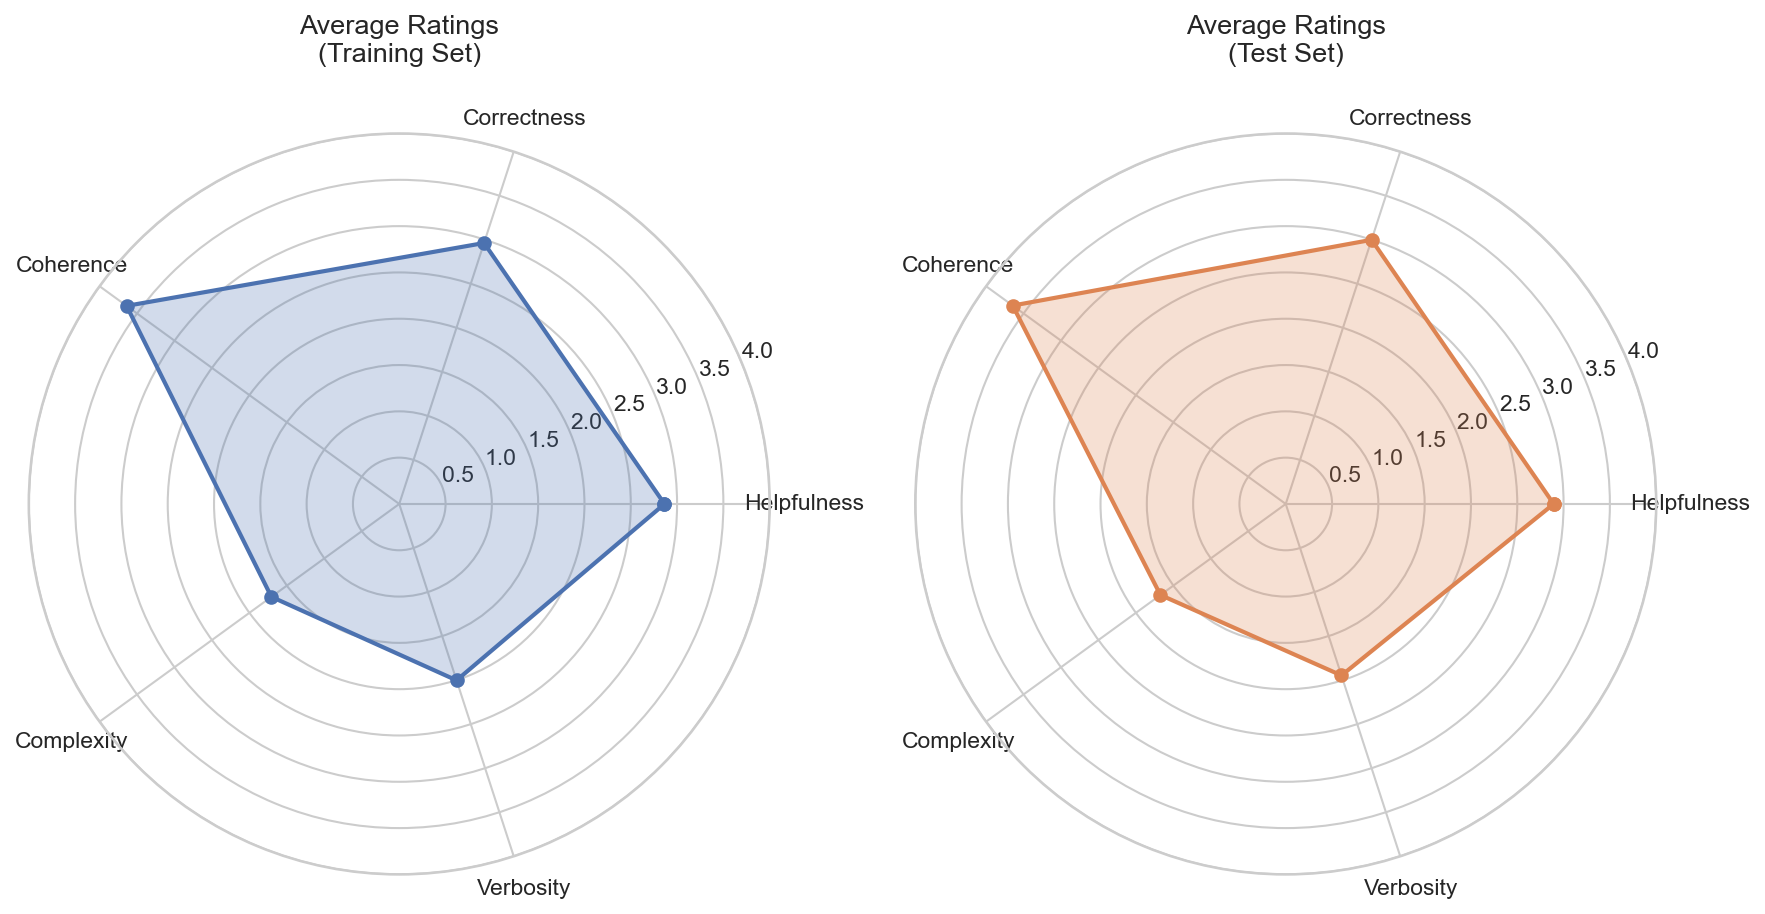
\includegraphics[width=\textwidth]{figures/average_ratings_radar.png}
  \captionof{figure}{Average ratings.}
  \label{fig:ratings_radar}
\end{minipage}
\end{figure}

\newpage
\subsection{Pair-Level Statistics}

\begin{figure}[htbp]
\centering
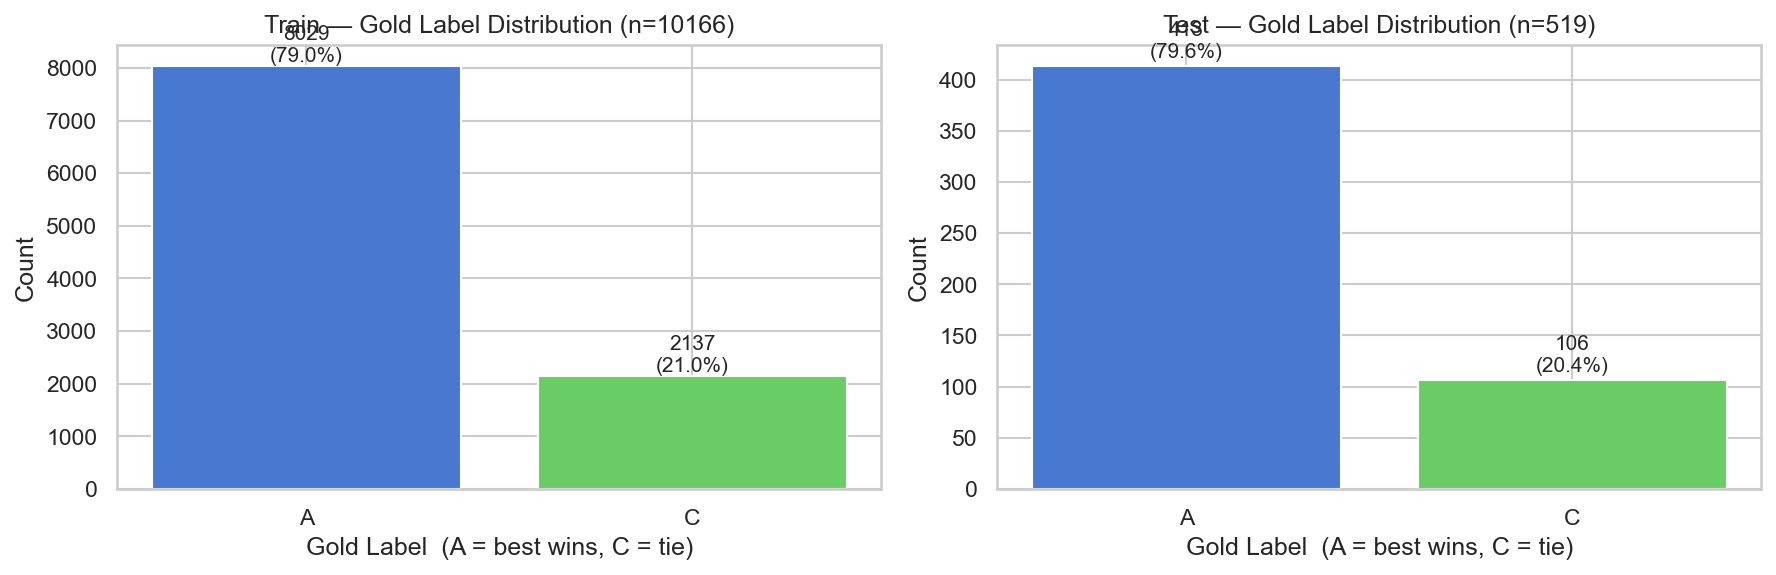
\includegraphics[width=0.7\textwidth]{figures/gold_label_distribution.png}
\caption{Gold label distribution. The better response is always placed as~A,
so the majority of labels are~A.}
\label{fig:gold}
\end{figure}

\begin{figure}[htbp]
\centering
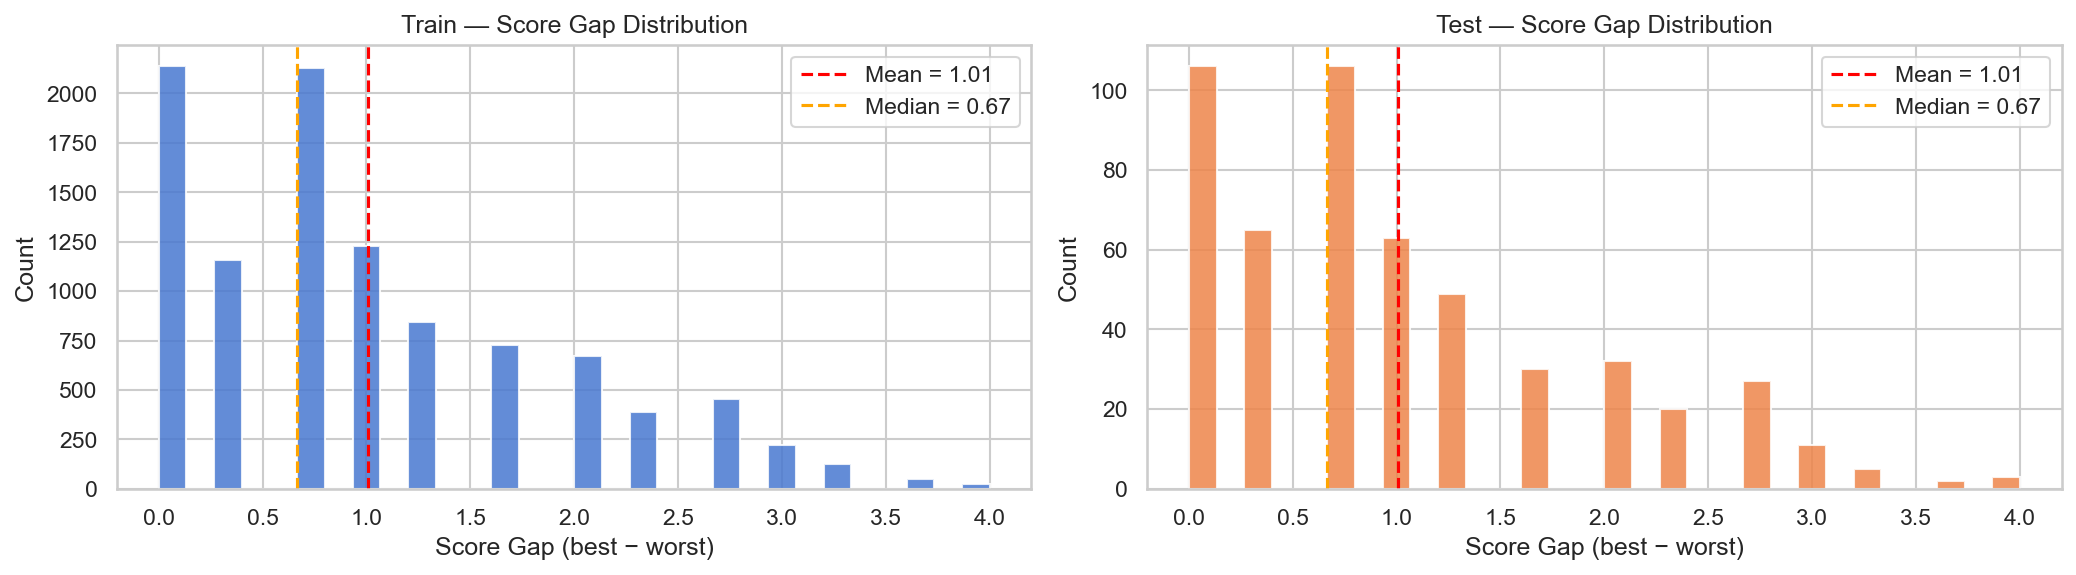
\includegraphics[width=0.75\textwidth]{figures/score_gap_histogram.png}
\caption{Composite score gap distribution. Smaller gaps indicate pairs that
are harder for a judge to distinguish.}
\label{fig:score_gap}
\end{figure}

\begin{figure}[htbp]
\centering
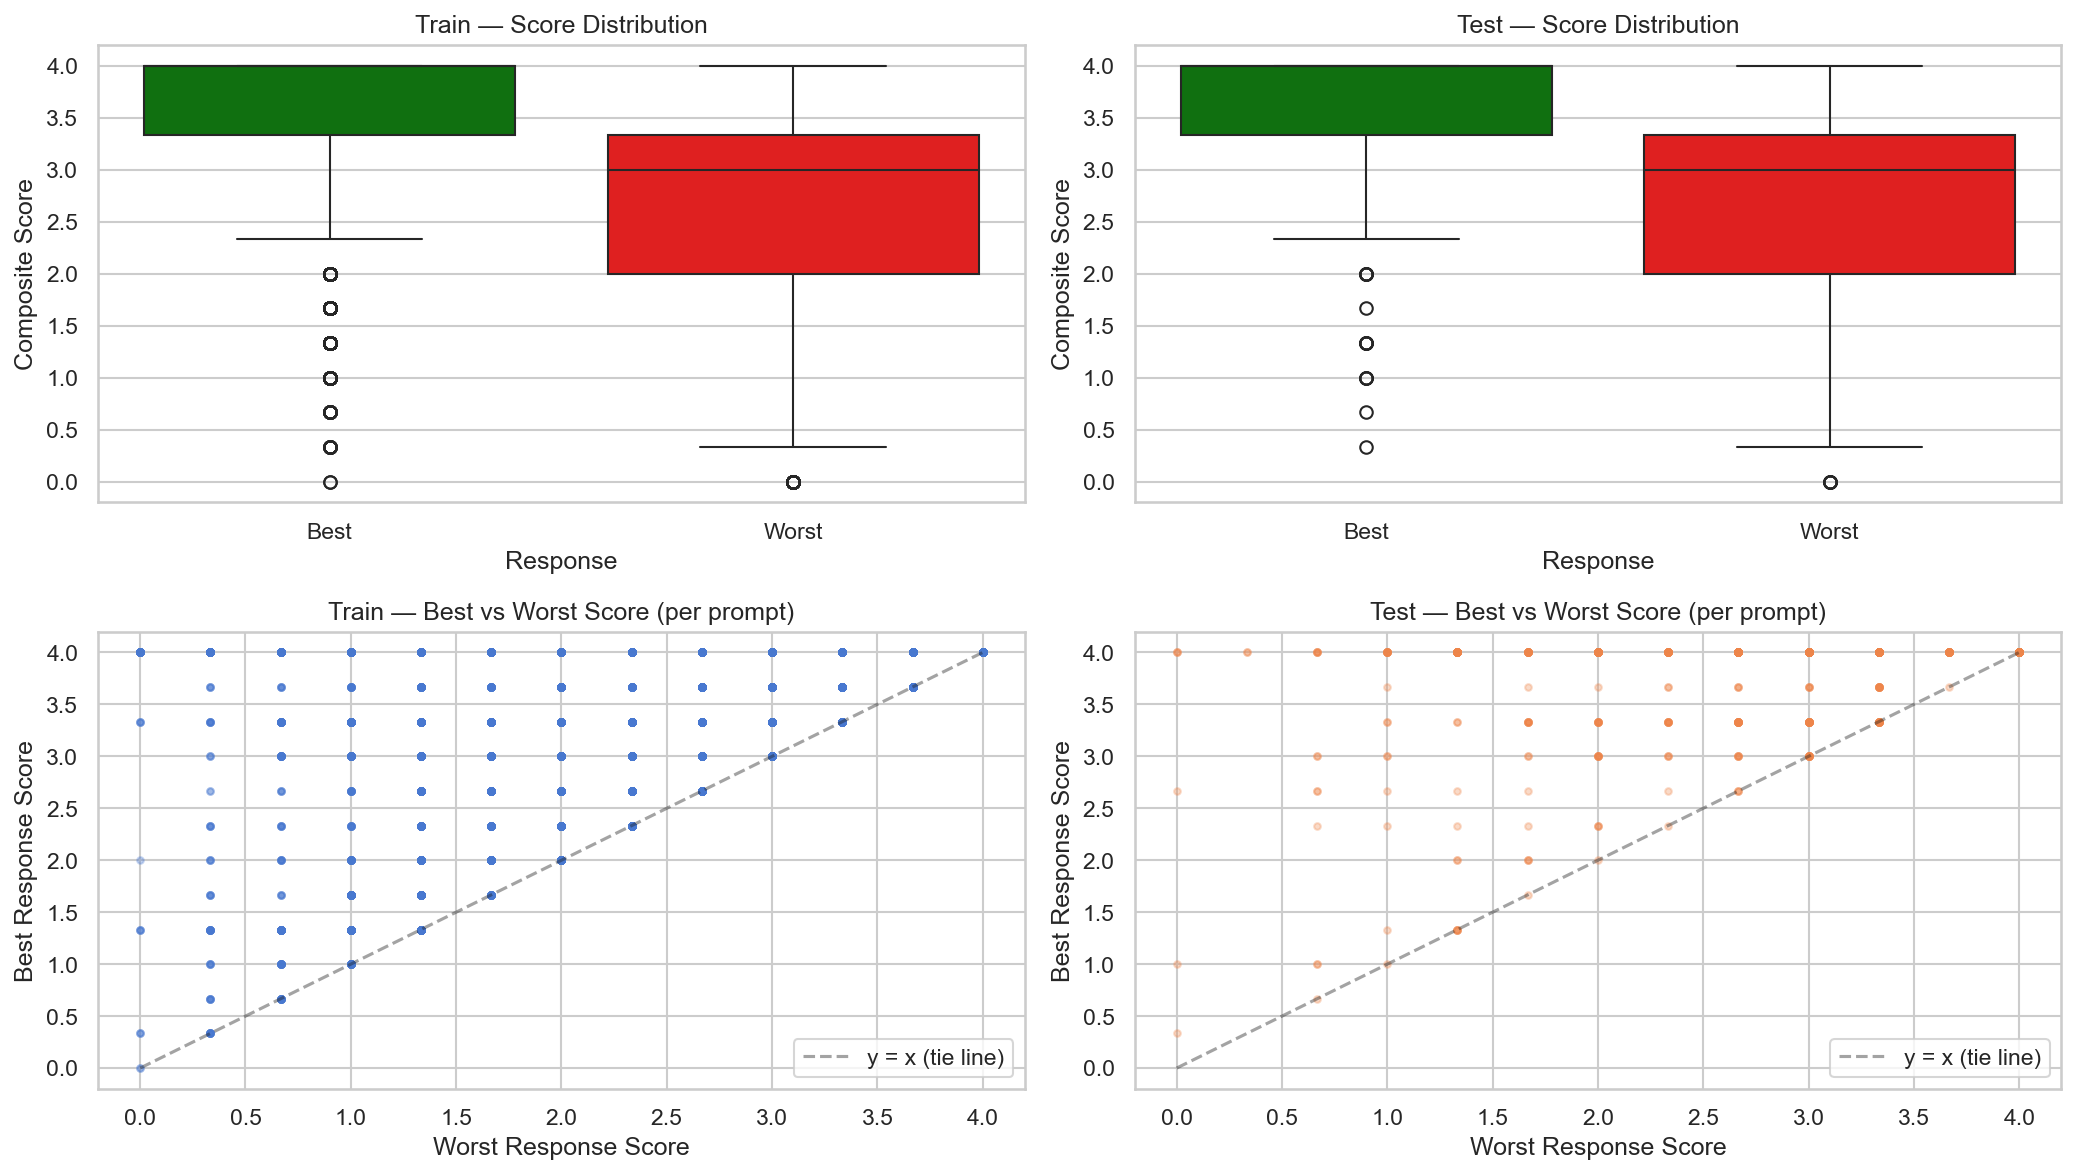
\includegraphics[width=0.65\textwidth]{figures/best_vs_worst_score.png}
\caption{Scatter plot of composite scores: response~A versus response~B.}
\label{fig:scatter}
\end{figure}


\begin{figure}[htbp]
\centering
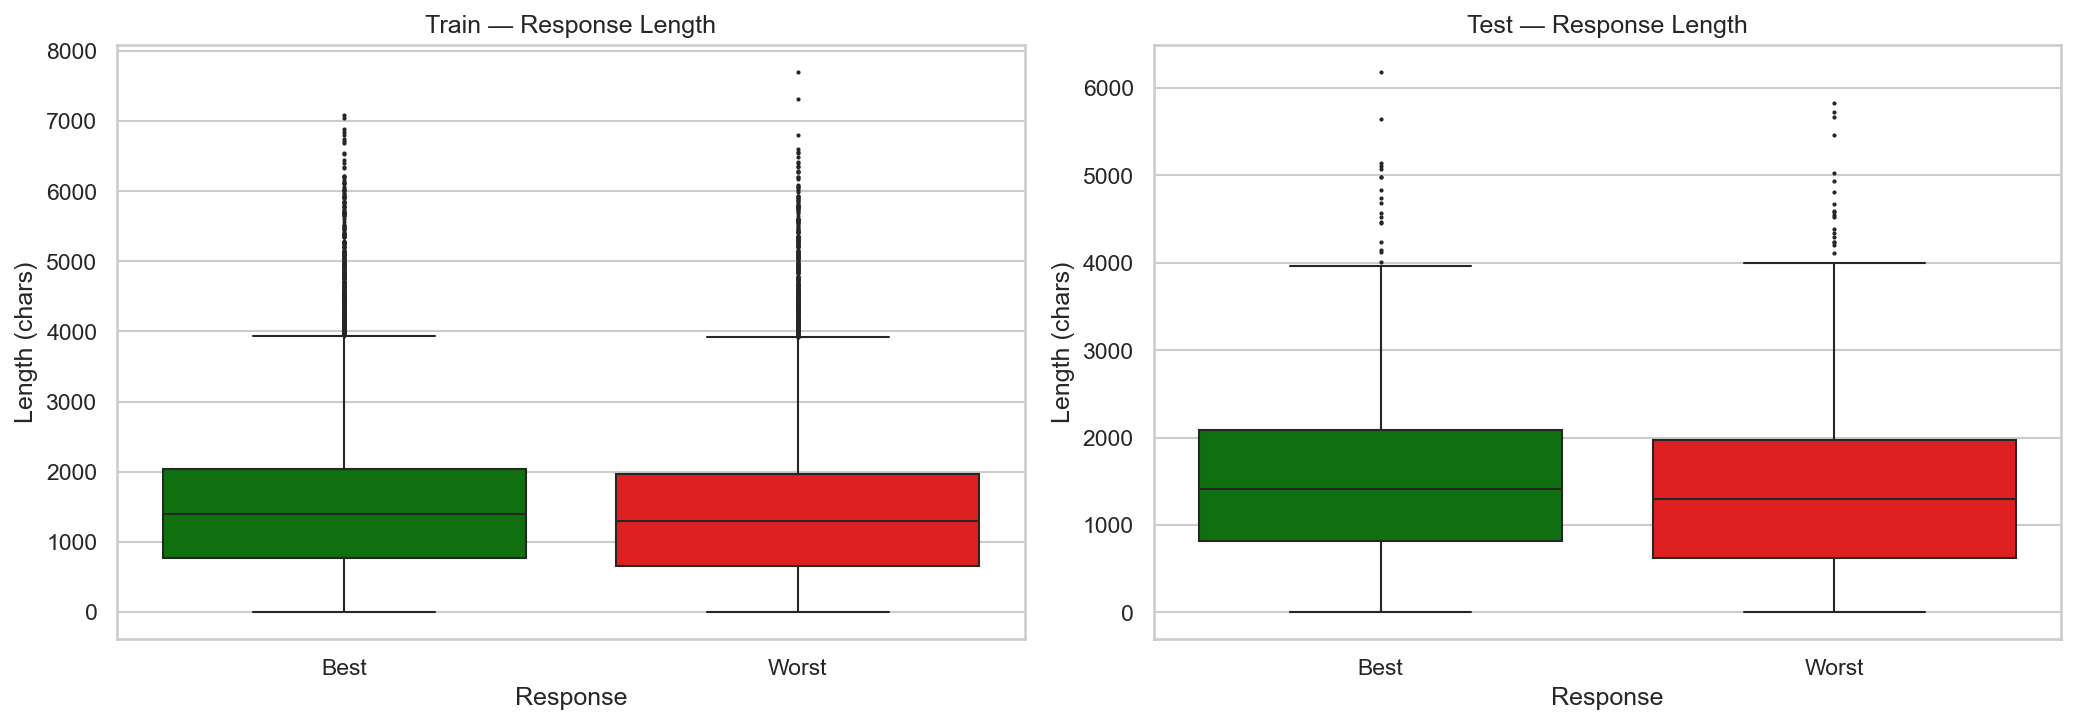
\includegraphics[width=0.75\textwidth]{figures/response_length_best_vs_worst.png}
\caption{Response length comparison between the better and worse response
in each pair.}
\label{fig:length_pair}
\end{figure}

\begin{figure}[htbp]
\centering
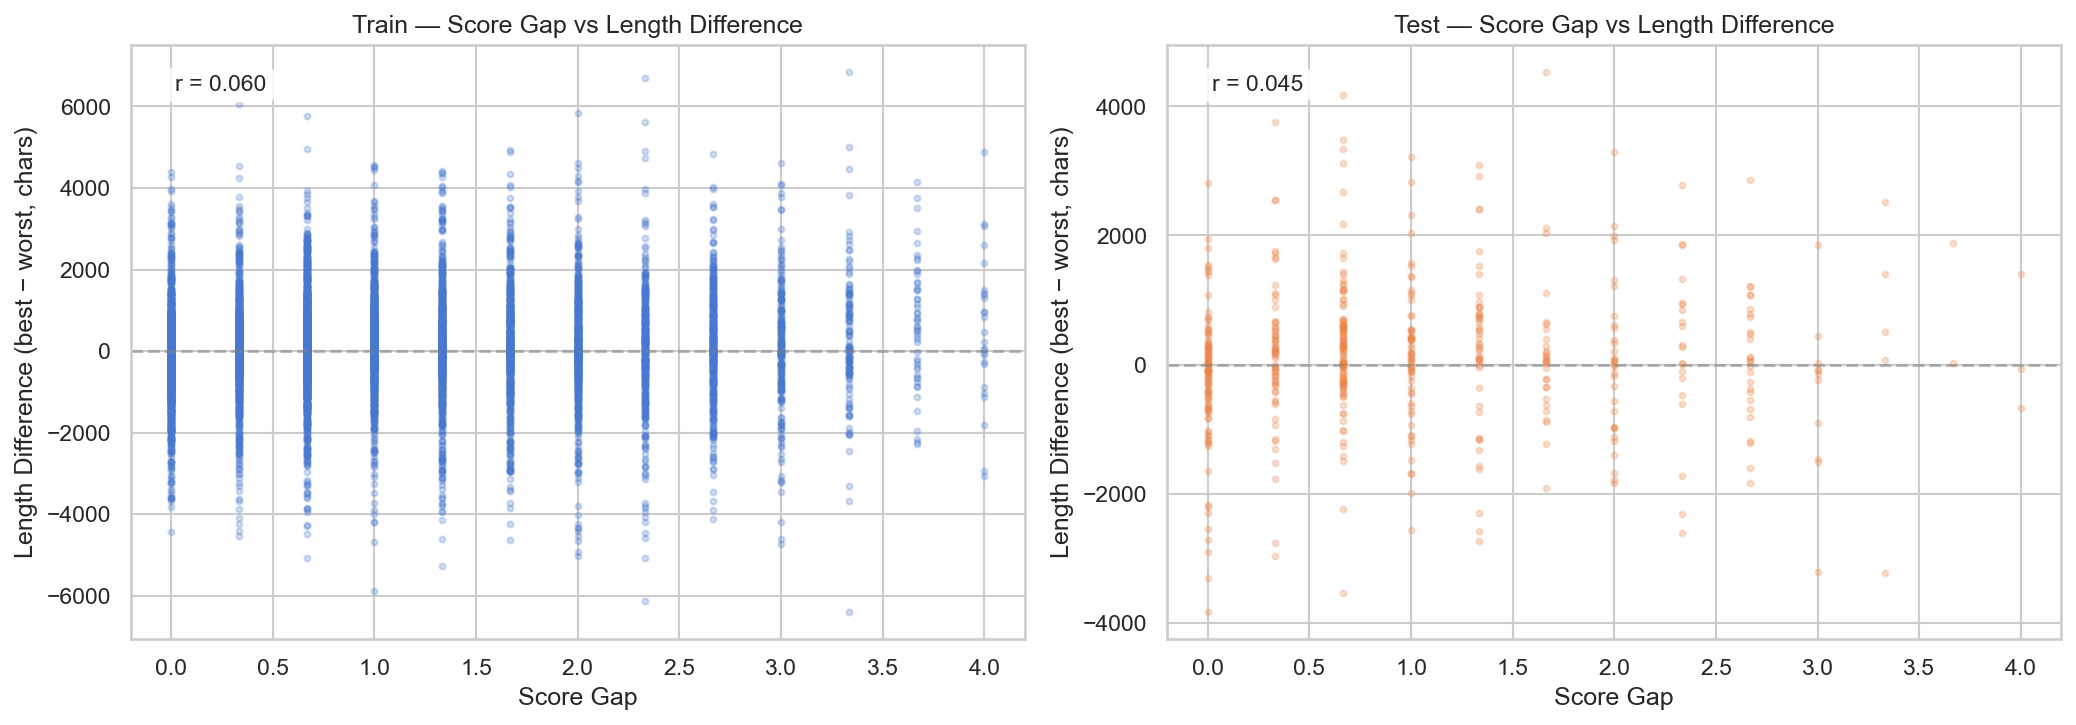
\includegraphics[width=0.7\textwidth]{figures/score_gap_vs_length_diff.png}
\caption{Score gap versus response length difference. Explores whether
quality differences correlate with verbosity differences.}
\label{fig:gap_length}
\end{figure}
\newpage
\subsection{Difficulty buckets}
\begin{figure}[htbp]
\centering
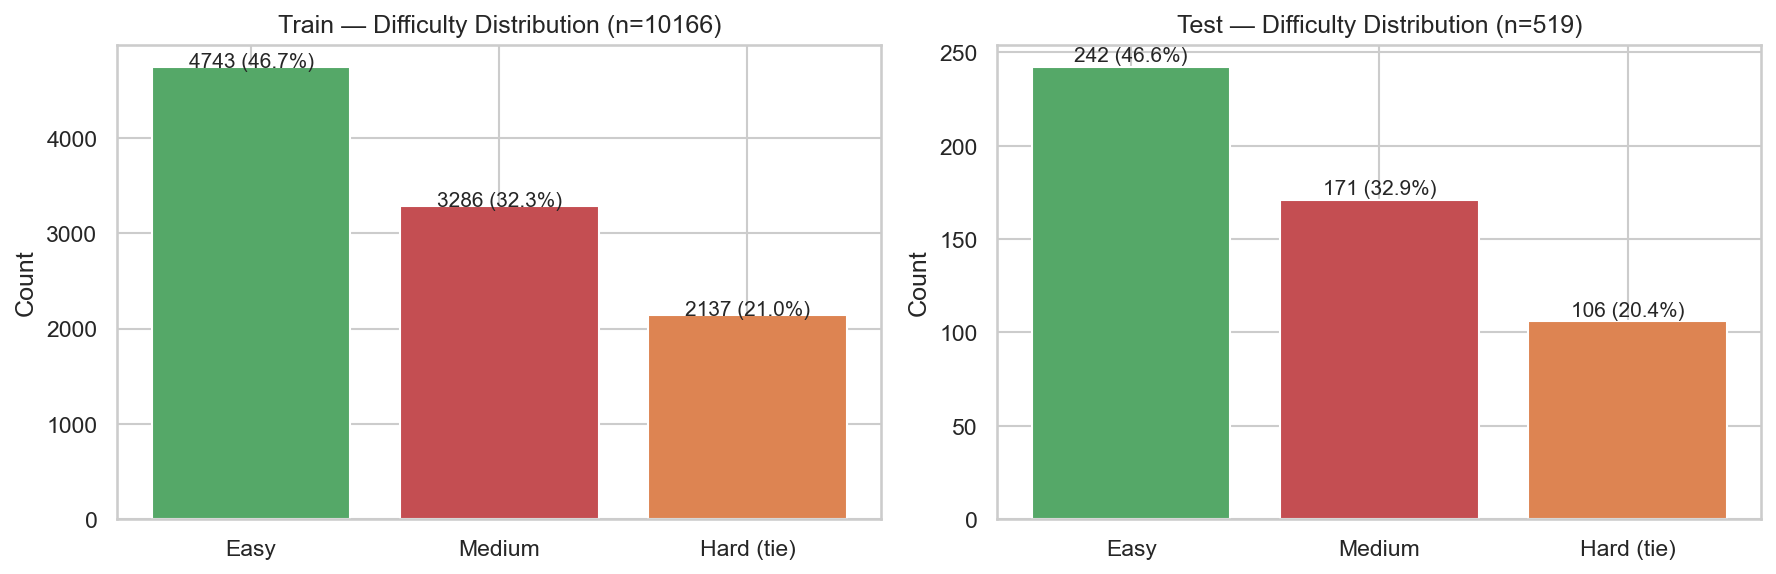
\includegraphics[width=0.65\textwidth]{figures/difficulty_buckets.png}
\caption{Number of pairs per difficulty bucket. Easy: gap~$> 1.0$;
medium: $0.33 < \text{gap} \leq 1.0$; hard: gap~$\leq 0.33$.}
\label{fig:difficulty}
\end{figure}


% ─────────────────────────────────────────────────────────────────────────────

\vfill
\begin{center}
\small\textit{End of document.}
\end{center}

\end{document}
